% ============================================================
%  chapters/ch05a.tex —— 第五章 超导性（前半）：§39–§45
%  印刷页 147–174（PDF 物理页 p158–p186）
%  插图：图 5（PDF p162，BCS 能谱；重绘 figures/fig5.pdf，图注照页面仅"图 5"无文字）
%        式(41.23) 费曼图块：无编号插图身份、原书为带公式编号的图形公式，
%        以 MinerU 裁剪图 figures/fig41_23.jpg + \tag{41.23} 排入（figures_manifest 18 幅之外）
%  圈码脚注标记：33 处（§39:4、§40:4、§41:5、§42:2、§43:2、§44:8、§45:8——
%    已全部排为 \footnote{...}（32 条脚注；§41 中"112 页的注解①"为跨页引用
%    字符，照排未动）。脚注文本由脚注代理按 300dpi 页面图逐页转录并自校；
%    原 p174①（求和公式）、p182①（两条 H_c 公式）两处 %%FN 注释已按页面
%    转录排入并删除（页面图比 OCR 原文多出引导句"为得出这个公式，我们写出"
%    与"在 BCS 模型中：…我们再得出…H_c 值："）
%  已修正的 OCR/原书错误（编号：依据页面 pNNN）：
%   1. p158 首锚点 %%p 157 系切片错位，§39 实起于 PDF p158（章首页"第五章 超导性"）；
%      自 %%p 158 起锚点与 PDF 页一致
%   2. p159 (39.1)(39.4) OCR \dagger → 照页面统一上标 +
%   3. p159 粒子数算符段 OCR 残句"件来确定化学势."，照页面补全"是粒子数算符；其次，
%      原则上可利用平均值 N̄ 等于给定系统中的粒子数这一条件来确定化学势."
%   4. p159–163 v_F OCR 误作 v_{\mathrm r}/\upsilon_{\mathrm r} 多处，照页面还原（39.7 后、
%      p–p_F 不等式、(39.19)、(39.21)、δp~Δ/v_F、(40.13) 前、ξ₀~ℏv_F/Δ₀ 等）
%   5. p160 (39.8) OCR \hat a^{*} → \hat a^{+}；(39.9) 末 OCR \hat B^-_{p+} → \hat B_p
%   6. p160 (39.13) OCR 仅存 v_p² 一行且带"⋅="，照页面还原为 u_p²、v_p² 两行加右花括号
%   7. p161 (39.14) OCR "\AA^{-1}" → ]^{-1}；(39.15) OCR \varrho → g
%   8. p161 (39.19) 后 OCR 漏句，照页面补"是费米面上单位能量间隔的粒子状态数
%      （νdε 是 dε 间隔内的状态数）."
%   9. p161 截断积分式 OCR "\mathrm dp^2\mathrm dp" → p²dp
%  10. p162 "耦合常数 θ 的幂展开；^g 包含在" → 照页面"耦合常数 g 的幂展开；g 包含在"；
%      色散律乱码 → ε=v_F|p−p_F|；段末杂噪"22"删除
%  11. p163 "这里当 Δ₀ ν_F 0 时 Δ₀ 变为零" → "这里当 ν_F→0 时 Δ₀ 变为零"（照页面）
%  12. p164 (40.3) OCR "7ζ(3θ)" → 7ζ(3)；(40.5) T_e → T_c
%  13. p165 (40.6) 前 n≈e^{−s/T̃} 乱码 → n≈e^{−ε/T}（照页面）
%  14. p166 (40.9) 后"(40.9)式的差值为 ~Δ²/μ"——页面即 Δ²/μ（无下标 0），照排；
%      (40.12) OCR C_s(T_c)/C_s(T_c) → C_s(T_c)/C_n(T_c)；S_{ν}, → S_s
%  15. p167 "只当 T_e~T 的值非常小" → "只当 T_c−T 的值非常小"；"比例 T³ 系数较小" →
%      "热容量与 T³ 成比例，比例系数较小"（均照页面）
%  16. p168 (41.1)(41.3) X_{\mathfrak n} → X_1；(41.11) OCR tag "1.11" → (41.11)，
%      F^{*} → F^{+}，OCR 乱尾"(4−π/2)F(X′,X′)"删除（页面无此内容）
%  17. p169 (41.9) OCR 四算符 ψ̂⁺_αψ̂⁺_γψ̂⁺_γψ̂_γ → 照页面三算符 ψ̂⁺_αψ̂⁺_γψ̂_γ（放大核实）；
%      方程前乱码上标删除
%  18. p170 (41.12) OCR \overleftrightarrow{Ξ} → Ξ；(41.16) \widetilde z → Ξ
%  19. p171 "δ(ω 王 ε)" → δ(ω±ε)；"将(41.9)式代入上式" → (41.19)（照页面）；
%      (41.20) 积分限照页面 ∬_{-∞}^{∞}
%  20. p172 (41.21)(41.22) δ 函数 OCR \hat\otimes/\hat s → δ
%  21. p172 §42 (A. A. ,. . ,1958) → （А.\,А.\,Абрикосов, Л.\,П.\,Горьков, 1958）（照页面）
%  22. p173 (42.1) 第二式 \hat{\overline\psi}^{a} → \hat{\overline\Psi}^{\mathrm M}；
%      "同 𝒢 一样" OCR "同 S-样" 还原；(42.6) ζ/ξ 混排 → ζ_s；(42.7) "𝒢(ζ,,p)" → 𝒢(ζ_s,p)
%  23. p175–176 §43 \hbar\omega_p → \hbar\omega_D（(43.1)–(43.3) 前后共 4 处）；
%      "量纲为 ^g 1" → "量纲为 1"；§44"液氮"→"液氦"（2 处，照页面）
%  24. p176 (44.2) 前 OCR"而j和∇Φ之间的关系归结为简单的正比 j, ∇Φ 关系" →
%      照页面"而 j_s 和 ∇Φ 之间的关系归结为简单的正比关系."
%  25. p177 "(见第三卷(111.9)式)\mathbb{O}_c" → ①；"(44.7) j=j ③…∇×" 段 OCR 错乱
%      重组照页面（"故 j=j_s③.现在对等式(44.7)两边施行 ∇× 运算"）
%  26. p178 (44.13) 及后文 \tilde\wp/\wp/\mathfrak s → 𝕵（\pmb{\mathfrak H}，照页面粗花体）；
%      "超导电子密度n→0" → n_s→0（照 p178–179）
%  27. p179 (44.15) OCR 乱尾照页面还原为 φ₀=πℏc/|e|=2×10⁻⁷ Gs·cm²（高斯·厘米²）
%  28. p180 习题解 M=−R⁵/(30δ)𝕵 → −R⁵/30δ²·𝕵（照页面）；"外场 𝕵" OCR \mathfrak{s} 还原
%  29. p181 (45.3) OCR \hbar/4m → \hbar²/4m（照页面）；(45.7) F_s−F_s → F_s−F_n；
%      "(见下面)② $\textcircled{2}$" 重复圈码删一
%  30. p182 (45.10) 原书排印 B²/2π（同页正文作"磁场能密度 B²/8π"，两处不一致），
%      照原书排入未改动，见遗留问题 a；"（I. Π.Горьков，1959）" →
%      （Л.\,П.\,Горьков, 1959）；p182 页底脚注①（两条 H_c 公式）窜入正文，
%      挪出为 %%FN 注释；p174 页底脚注①（求和公式）同此（%%FN p174）
%  31. p185 (B.Ⅱ.金兹堡，I.Ⅱ.朗道) → （В.\,Л.\,金兹堡, Л.\,Д.\,朗道）；习题 B(y) 分母
%      OCR "cosh(cosh(dθ/2δ))" → cosh(dθ/2δ)、分子 "y²·(∂d/2)²" → y²−(d/2)²（照页面）
%  32. p186 各式 𝕵（\tilde\wp/\wp）还原；B″=θ²B/δ²、ψ₀²=|a|/b 照页面
%  33. 各页行尾杂散字符（"X D""小H""2 D""22"等）删除；直引号照中文弯引号还原
%  遗留问题：
%   a. (45.10) B²/2π 与同页正文 B²/8π 不一致（疑原书排印之误），照原书排入，待主控裁定
%   b. p178 "∇×(∇×)B=−ΔB" 括号位置照原书排入（疑脱 B 于括号内），未改动
%   c. (43.2) 前一句"(做代替 ε̃~μ)."之"做"字照页面排入
%   d. 圈码脚注已全部排入（32 条 \footnote + 1 处跨页引用照排）；
%      各页脚注数与页面图逐一核对（p159/160/162/166/171/173/184 无脚注）
%   e. (41.23) 费曼图暂用 MinerU 裁剪图（jpg），如后续统一重绘可换 fig41_23.pdf
% ============================================================
\chapter{超导性}

\section{超流费米气体\ 能谱}

在第一章所叙述的朗道理论都只与一种费米液体有关，即只与不产生超流现象而有能谱的液体有关. 对于量子费米液体来说，这种谱型并不是唯一可能的，现在我们开始研究具有另一类型能谱的费米系统. 采用粒子间有吸引作用的简并近理想费米气体的简单模型（这是可以作完全的理论研究的），可以最鲜明地说明这种能谱的起源及其基本性质\footnote{这个问题是超导理论的基础，该理论是由~J.\,Bardeen, L.\,N.\,Cooper 和~J.\,R.\,Schrieffer 于（1957）建立的. 下面叙述的解法属于~Н.\,Н.\,Боголюбов（1958）的工作.}.

粒子间呈现排斥作用的弱非理想费米气体已在§6中讨论过了. 初看起来，在那一节里所进行的计算，对于粒子间的排斥作用情况和吸引作用情况（即散射长度$a$为正值和负值时）在同等程度上都是正确的. 但实际上，在吸引作用（$a<0$）的情况下，用这种方法求出的系统的基态，对于一定的改组（改变基态的性质和降低能量）是不稳定的.

这种不稳定性的物理本质在于粒子都倾向于“成对”：在$\bm p$空间中，位于费米面附近并具有大小相等、方向相反动量和反平行自旋的粒子对，都倾向于形成束缚态，这就是所谓的库珀（L.\,N.\,Cooper, 1957）效应. 奇妙的是，在费米气体中粒子间的吸引作用无论有多弱都会产生这种效应.

正是由于这种效应，在讨论有排斥作用的费米气体问题中曾使用过的适于气体单个粒子自由态的算符集合$\hat a_{p\alpha},\hat a^{+}_{p\alpha}$，现在已不能作为微扰论最初的正确近似了\footnote{指出微扰论（就§6中运用的形式来说）不适于具有自旋投影为~$\pm1/2$ 和动量为~$\bm p_2\approx-\bm p_1$ 的粒子对，也就指明~$\vartheta=\pi$ 处存在奇点，用这种理论得到的准粒子相互作用函数的表达式(6.16)就具有这种奇点；这种奇点只在反平行自旋的情况下才存在，而这些自旋对应于算符~$\bm\sigma_1\bm\sigma_2$ 的本征值等于$-3$.}. 现在需要立即引入新的算符来代替上述算符，我们寻求的是下列线性组合形式的算符：
\begin{equation}
\begin{aligned}
\hat b_{p-} &= u_p\,\hat a_{p-} + v_p\,\hat a^{+}_{-p,+}\,,\\
\hat b_{p+} &= u_p\,\hat a_{p+} - v_p\,\hat a^{+}_{-p,-}\,,
\end{aligned}
\label{39.1}
\end{equation}
上述形式合并了具有相反动量和相反自旋（投影）的粒子的算符（下标$+$和$-$表示自旋投影的两个值）；由于气体是各向同性的，系数$u_p,v_p$只能依赖于动量$\bm p$的绝对值. 为使这些新算符对应于准粒子的产生和湮没，它们应同以前的算符一样遵从同样的费米对易规则：
\begin{equation}
\hat b_{p\alpha}\hat b^{+}_{p\alpha} + \hat b^{+}_{p\alpha}\hat b_{p\alpha} = 1\,,
\label{39.2}
\end{equation}
而所有其它的算符对都是反对易的（下标$\alpha$注明两个自旋投影值）. 对此，变换系数应遵从如下条件：
\begin{equation}
u_p^2 + v_p^2 = 1
\label{39.3}
\end{equation}
（适当地选择相因子能够使$u_p,v_p$都成为实数）. 这时，对\eqref{39.1}式的逆变换具有如下形式：
\begin{equation}
\begin{aligned}
\hat a_{p+} &= u_p\,\hat b_{p+} + v_p\,\hat b^{+}_{-p,-}\,,\\
\hat a_{p-} &= u_p\,\hat b_{p-} - v_p\,\hat b^{+}_{-p,+}\,.
\end{aligned}
\label{39.4}
\end{equation}
根据同样原因（具有相反动量和相反自旋的一列粒子之间的相互作用起主要作用），在哈密顿量(6.7)的第二个求和式中，我们只保留$\bm p_1=-\bm p_2\equiv\bm p$，$\bm p'_1=-\bm p'_2\equiv\bm p'$的一些项：
\begin{equation}
\hat H = \sum_{p\alpha}\frac{p^2}{2m}\hat a^{+}_{p\alpha}\hat a_{p\alpha}
- \frac{g}{V}\sum_{pp'}\hat a^{+}_{p'+}\hat a^{+}_{-p',-}\hat a_{-p,-}\hat a_{p+}\,,
\label{39.5}
\end{equation}
式中重新引入了“耦合常数”$g=4\pi\hbar^2|a|/m$（散射长度$a<0$）.

在以下的计算中，最好再一次采用通常的方法，不必明显考虑系统中粒子数的不变性：现在引入差$\hat H'=\hat H-\mu\hat N$作为新哈密顿量，这里
\begin{equation*}
\hat N = \sum_{p\alpha}\hat a^{+}_{p\alpha}\hat a_{p\alpha}
\end{equation*}
是粒子数算符；其次，原则上可利用平均值$\bar N$等于给定系统中的粒子数这一条件来确定化学势.

我们还引入记号
\begin{equation}
\eta_p = \frac{p^2}{2m} - \mu\,,
\label{39.6}
\end{equation}
因为$\mu=p_{\mathrm F}^2/2m$，所以在费米面附近
\begin{equation}
\eta_p = v_{\mathrm F}(p - p_{\mathrm F})\,,
\label{39.7}
\end{equation}
式中$v_{\mathrm F}=p_{\mathrm F}/m$. 从表达式\eqref{39.5}减去$\mu\hat N$，于是我们把原哈密顿量写为
\begin{equation}
\hat H' = \sum_{p\alpha}\eta_p\hat a^{+}_{p\alpha}\hat a_{p\alpha}
- \frac{g}{V}\sum_{pp'}\hat a^{+}_{p'+}\hat a^{+}_{-p',-}\hat a_{-p,-}\hat a_{p+}\,.
\label{39.8}
\end{equation}

我们在这个哈密顿量中进行\eqref{39.4}式的变换. 利用关系式\eqref{39.2}—\eqref{39.3}和可把求和下标$\bm p$换成$-\bm p$，得到：
\begin{equation}
\begin{aligned}
\hat H' ={}& 2\sum_p\eta_p v_p^2 + \sum_p\eta_p\bigl(u_p^2 - v_p^2\bigr)\bigl(\hat b^{+}_{p+}\hat b_{p+} + \hat b^{+}_{p-}\hat b_{p-}\bigr) + {}\\
&+\ 2\sum_p\eta_p u_pv_p\bigl(\hat b^{+}_{p+}\hat b^{+}_{-p,-} + \hat b_{-p,-}\hat b_{p+}\bigr) - \frac{g}{V}\sum_{p,p'}\hat B^{+}_{p'}\hat B_p
\end{aligned}
\label{39.9}
\end{equation}
\begin{equation*}
\hat B_p = u_p^2\,\hat b_{-p,-}\hat b_{p+} - v_p^2\,\hat b^{+}_{p+}\hat b^{+}_{-p,-}
+ v_pu_p\bigl(\hat b_{-p,-}\hat b^{+}_{-p,-} - \hat b^{+}_{p+}\hat b_{p+}\bigr)\,.
\end{equation*}

在熵一定时，利用系统能量$E$取最小值的条件来选择系数$u_p,v_p$. 熵由组合表达式来定义；
\begin{equation*}
S = -\sum_{p\alpha}\bigl[n_{p\alpha}\ln n_{p\alpha} + (1-n_{p\alpha})\ln(1-n_{p\alpha})\bigr]\,.
\end{equation*}
因此上述条件与在准粒子占有数$n_{p\alpha}$一定时能量取最小值是等价的.

在哈密顿量\eqref{39.9}中，对角矩阵元只具有含乘积
\begin{equation*}
\hat b^{+}_{p\alpha}\hat b_{p\alpha} = n_{p\alpha}\,,\quad \hat b_{p\alpha}\hat b^{+}_{p\alpha} = 1 - n_{p\alpha}
\end{equation*}
的一些项. 因此我们求得：
\begin{equation}
\begin{aligned}
E ={}& 2\sum_p\eta_p v_p^2 + \sum_p\eta_p\bigl(u_p^2 - v_p^2\bigr)(n_{p+} + n_{p-}) - {}\\
&-\ \frac{g}{V}\Biggl[\sum_p u_pv_p\bigl(1 - n_{p+} - n_{p-}\bigr)\Biggr]^2\,.
\end{aligned}
\label{39.10}
\end{equation}
把这个表达式对参数$u_p$［这时考虑\eqref{39.3}的关系］取变分，我们便得到极小值的条件：
\begin{equation*}
\frac{\delta E}{\delta u_p} = -\frac{2}{v_p}\bigl(1 - n_{p+} - n_{p-}\bigr)\Biggl[2\eta_pu_pv_p
- \frac{g}{V}\bigl(u_p^2 - v_p^2\bigr)\sum_{p'}u_{p'}v_{p'}\bigl(1 - n_{p'+} - n_{p'-}\bigr)\Biggr] = 0\,,
\end{equation*}
从而求得方程
\begin{equation}
2\eta_pu_pv_p = \Delta\bigl(u_p^2 - v_p^2\bigr)\,,
\label{39.11}
\end{equation}
式中$\Delta$表示求和：
\begin{equation}
\Delta = \frac{g}{V}\sum_p u_pv_p\bigl(1 - n_{p+} - n_{p-}\bigr)\,.
\label{39.12}
\end{equation}
由\eqref{39.11}和\eqref{39.3}式，通过$\eta_p$和$\Delta$表达$u_p,v_p$：
\begin{equation}
\left.\begin{matrix} u_p^2 \\ v_p^2 \end{matrix}\right\}
= \frac{1}{2}\Biggl(1 \pm \frac{\eta_p}{\sqrt{\Delta^2 + \eta_p^2}}\Biggr).
\label{39.13}
\end{equation}
将这两个值代入\eqref{39.12}式，即得到确定$\Delta$的方程：
\begin{equation*}
\frac{g}{2V}\sum_p\frac{1 - n_{p+} - n_{p-}}{\sqrt{\Delta^2 + \eta_p^2}} = 1\,.
\end{equation*}
在热平衡的情况下，准粒子占有数与自旋方向无关并由费米分布（化学势等于零，见6页的注解）给出：
\begin{equation}
n_{p+} = n_{p-} \equiv n_p = \bigl[\mathrm e^{\varepsilon/T} + 1\bigr]^{-1}.
\label{39.14}
\end{equation}
再将求和变为对$\bm p$空间求积分，我们把这个方程写成
\begin{equation}
\frac{g}{2}\int\frac{1 - 2n_p}{\sqrt{\Delta^2 + \eta_p^2}}\ \frac{\mathrm d^3p}{(2\pi\hbar)^3} = 1\,.
\label{39.15}
\end{equation}

现在转而研究上面得出的几个关系式. 我们看到，量$\Delta$在所研究类型的能谱理论中起主要作用. 现在首先计算$T=0$时这个量的数值（用$\Delta_0$表示）.

当$T=0$时，准粒子是不存在的，因此$n_p=0$，方程\eqref{39.15}取如下形式：
\begin{equation}
\frac{g}{2(2\pi\hbar)^3}\int\frac{4\pi p^2\,\mathrm dp}{\sqrt{\Delta_0^2 + \eta_p^2}} = 1\,.
\label{39.16}
\end{equation}
应立即指出，当$g<0$时，即在粒子间呈现排斥作用的情况下（方程两边的符号显然是不同的），这个方程显然不可能有$\Delta_0$的解.

满足$\Delta_0\ll v_{\mathrm F}|p_{\mathrm F}-p|\ll v_{\mathrm F}p_{\mathrm F}\sim\mu$的动量区域对\eqref{39.16}式中的积分提供主要贡献，并且积分具有对数性质（结果证实$\Delta_0$比$\mu$小）. 当某一$\eta=\tilde\varepsilon\sim\mu$时截断对数积分，我们有\footnote{当~$p\gg p_{\mathrm F}$ 时~$\eta_p\propto p^2$，因而(39.16)式中的积分就写出的形式来看，将同~$p$ 一样发散. 但实际上这个发散是虚假的，将常数~$g$（即散射长度~$a$）和相互作用势之间的关系重整化，即可消除此发散，这和§6及§25中的处理方法是一样的. 连续进行这样相当复杂的计算还可以求出截断参数~$\tilde\varepsilon$ 和化学势~$\mu$ 之间的比例系数：$\tilde\varepsilon=(2/e)^{7/3}\mu=0.49\mu$［参看~Л.\,П.\,Горьков, Т.\,К.\,Мелик-Бархударов, ЖЭТФ, 40, 1452 (1961)］.}
\begin{equation*}
\int\frac{p^2\,\mathrm dp}{\bigl[\Delta_0^2 + v_{\mathrm F}^2(p_{\mathrm F}-p)^2\bigr]^{1/2}}
\approx \frac{p_{\mathrm F}^2}{v_{\mathrm F}}\int\frac{\mathrm d\eta}{(\Delta_0^2 + \eta^2)^{1/2}}
\approx \frac{2p_{\mathrm F}^2}{v_{\mathrm F}}\ln\frac{\tilde\varepsilon}{\Delta_0}\,.
\end{equation*}
因此求得：
\begin{equation}
\frac{gmp_{\mathrm F}}{2\pi^2\hbar^3}\ln\frac{\tilde\varepsilon}{\Delta_0} = 1\,.
\label{39.17}
\end{equation}
从而
\begin{equation}
\Delta_0 = \tilde\varepsilon\exp\Biggl(-\frac{2\pi^2\hbar^3}{gmp_{\mathrm F}}\Biggr)
= \tilde\varepsilon\exp\Biggl(-\frac{\pi\hbar}{2p_{\mathrm F}|a|}\Biggr)\,,
\label{39.18}
\end{equation}
这个表达式也可以写成
\begin{equation}
\Delta_0 = \tilde\varepsilon\exp(-2/g\nu_{\mathrm F})\,,
\label{39.19}
\end{equation}
式中$\nu_{\mathrm F}=mp_{\mathrm F}/\pi^2\hbar^3$是费米面上单位能量间隔的粒子状态数（$\nu\,\mathrm d\varepsilon$是$\mathrm d\varepsilon$间隔内的状态数）.

使我们最感兴趣的是系统能谱即元激发能量$\varepsilon_{p+}=\varepsilon_{p-}\equiv\varepsilon(p)$的形式. 现在我们根据准粒子占有数改变时整个系统能量的变化［即把\eqref{39.10}式中的$E$对$n_{p\alpha}$取变分］来求$\varepsilon(\bm p)$的形式. 因为$u_p,v_p$的值已由$E$对它们的微商等于零这一条件选定了，所以可在$u_p,v_p$一定的情况下把$E$对$n_{p\alpha}$取变分. 因此
\begin{equation*}
\varepsilon = \Biggl(\frac{\delta E}{\delta n_{p\alpha}}\Biggr)_{u_pv_p}\,,
\end{equation*}
利用\eqref{39.11}—\eqref{39.13}式计算微商，便得到如下简单的结果：
\begin{equation}
\varepsilon(p) = \sqrt{\Delta^2 + \eta_p^2}\,.
\label{39.20}
\end{equation}

\par\nopagebreak\noindent\begin{minipage}{\linewidth}\centering
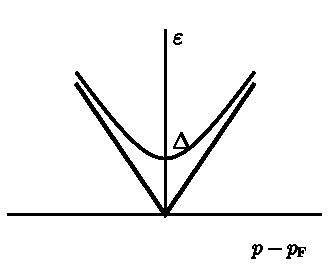
\includegraphics[width=5cm]{fig5.pdf}\\[0.3em]
{\small 图\ 5}
\end{minipage}\par\nopagebreak

我们看到，准粒子能量不可能小于$p=p_{\mathrm F}$时所达到的$\Delta$值. 换言之，系统的激发态与基态隔着一个能隙. 具有半整数自旋时，准粒子都必定成对出现. 就此意义可以说，能隙的大小等于$2\Delta$. 我们注意到这是一个指数函数性的小量：因为$p_{\mathrm F}\ln|a|/\hbar\ll1$，所以与$\mu$相比$\Delta_0$是指数函数小量. 也应指出，表达式\eqref{39.18}不可能按小参数——耦合常数$g$的幂展开；$g$包含在指数函数的指数的分母中，因此$g=0$的值是函数$\Delta_0(g)$的本性奇点.

\eqref{39.20}式的能谱遵从§23中建立的超流条件：$\varepsilon/p$的最小值不等于零. 因此粒子间相互吸引的费米气体必定具有超流性质.

在图5中将超流情况下准粒子的色散规律（上面的曲线）和正常费米系统的色散规律作了对比. 在后一种情况下，这种规律（根据§1结尾所作的解释）是用$\varepsilon=v_{\mathrm F}|p-p_{\mathrm F}|$的两条直线表示出来的.

能隙$\Delta$的大小与温度有关，这就是说能谱形式本身与准粒子的统计分布有关——与正常型费米液体的情况类似. 因为当温度升高时准粒子占有数增加（趋于1），所以从方程\eqref{39.15}就可以看出，这时$\Delta$减小并在某一有限温度$T_{\mathrm c}$时变为零：系统由超流状态变成正常状态. 这个转变点就是第二级相变（类似于超流玻色液体的$\lambda$转变）.

在简并费米气体的能谱中有能隙存在，它是本节开头已经讲到的“成对”效应的表现. $2\Delta$的大小可以看作是库珀对的束缚能，即分离这种粒子对时所需的能量.

哈密顿量\eqref{39.5}（如§6所指出的）只考虑s单态（即粒子的相对运动轨道角动量等于零，并且自旋反向平行）上粒子对间的相互作用. 总自旋等于零时，粒子对的行为同玻色型组成物一样能够以任意数目\footnote{原文为有限数目——译者注.}聚集在（整体运动的）最低能级（即总动量为零的能级）. 就这样的直观解释来看，这种现象完全类似于玻色气体中粒子在零能态的聚集（玻色-爱因斯坦凝聚）；在这种情况下，凝聚体是成对粒子的集合.

当然不应赋予束缚对的概念以过多的字面上的意义. 更准确地说，应该谈及$\bm p$空间中粒子对各态之间的关联，这种关联使合动量为零的粒子对以有限概率出现. 在关联区域内，动量的弥散值$\delta p$对应于$\Delta$量级的能量，即$\delta p\sim\Delta/v_{\mathrm F}$. 相应长度$\xi\sim\hbar/\delta p\sim\hbar v_{\mathrm F}/\Delta$，用来确定具有关联动量的粒子之间距离的数量级. 当$T=0$时，这个长度（称作相干长度）为
\begin{equation}
\xi_0\sim\frac{\hbar v_{\mathrm F}}{\Delta_0}\sim\frac{\hbar}{p_{\mathrm F}}\exp\Biggl(\frac{\pi\hbar}{2p_{\mathrm F}|a|}\Biggr).
\label{39.21}
\end{equation}
因为对简并费米气体$\hbar/p_{\mathrm F}$在数量级上与原子间距相同，所以我们看到，$\xi_0$比原子间距大得多. 特别是，这种情况直观地表明了束缚对的概念不是无条件的.

库珀效应的发生与费米面的存在有密切关系，该面$T=0$时在$\bm p$空间的占据状态限定了有限区域；有一个重要情况是：在这个表面上，单位能量间隔的状态数不等于零. 这种关系表现于决定能隙$\Delta_0$大小的公式\eqref{39.19}之中，这里当$\nu_{\mathrm F}\to0$时$\Delta_0$变为零.

\section{超流费米气体\ 热力学性质}

{\emergencystretch=1.5em 现在我们从计算能隙大小与温度的关系来着手研究超流费米气体的热力学性质. 把方程\eqref{39.15}重写成如下形式：\par}
\begin{equation*}
-1 + \frac{g}{2}\int\frac{\mathrm d^3p}{\varepsilon(2\pi\hbar)^3} = g\int\frac{n_p\,\mathrm d^3p}{\varepsilon(2\pi\hbar)^3}\,.
\end{equation*}
我们注意到，方程左边的积分与$T=0$时积分的差别，仅在于把$\Delta_0$换成$\Delta$. 因此考虑到\eqref{39.17}式我们看出，方程左边等于$\dfrac{gp_{\mathrm F}m}{2\pi^2\hbar^3}\ln\dfrac{\Delta_0}{\Delta}$. 把\eqref{39.14}式中的$n_p$代入方程的右边并对$\mathrm dp=\mathrm d\eta/v_{\mathrm F}$进行积分：
\begin{equation}
\ln\frac{\Delta_0}{\Delta} = \int_{-\infty}^{\infty}\frac{\mathrm d\eta}{\varepsilon(\mathrm e^{\varepsilon/T}+1)} \equiv 2I\Biggl(\frac{\Delta}{T}\Biggr),
\label{40.1}
\end{equation}
式中
\begin{equation*}
I(u) = \int_0^{\infty}\frac{\mathrm dx}{\sqrt{x^2+u^2}\,\bigl(\exp\sqrt{x^2+u^2}+1\bigr)}
\end{equation*}
（由于积分收敛得很快，积分限可以扩大到$\pm\infty$）.

在低温（$T\ll\Delta_0$）范围内容易算出积分\footnote{当~$u$很大时，$I(u)$按~$1/u$的展开式的第一项为：
\begin{equation*}
I(u)\approx\int_0^{\infty}\frac{\mathrm dx}{u}\exp\Biggl[-u\Biggl(1+\frac{x^2}{2u^2}\Biggr)\Biggr]=\Biggl(\frac{\pi}{2u}\Biggr)^{\!1/2}\mathrm e^{-u}.
\end{equation*}}，并得到：
\begin{equation}
\Delta = \Delta_0\Biggl(1 - \sqrt{\frac{2\pi T}{\Delta_0}}\,\mathrm e^{-\Delta_0/T}\Biggr).
\label{40.2}
\end{equation}
但在相变点附近区域内$\Delta$很小，于是积分$I(\Delta/T)$展开式的前几项给出\footnote{对于积分~$I(u)$的展开式来说，当~$u\to0$时我们可以从展开式中加上和减去如下积分：
\begin{equation*}
I_1=\frac{1}{2}\int_0^{\infty}\Biggl(\frac{1}{\sqrt{x^2+u^2}}-\frac{1}{x}\tanh\frac{x}{2}\Biggr)\mathrm dx,
\end{equation*}
于是~$I=I_1+I_2$，其中
\begin{equation*}
I_2=\frac{1}{2}\int_0^{\infty}\Biggl(\frac{1}{x}\tanh\frac{x}{2}-\frac{1}{\sqrt{x^2+u^2}}\tanh\frac{\sqrt{x^2+u^2}}{2}\Biggr)\mathrm dx.
\end{equation*}
在~$I_1$中可以简单地求出第一项的积分，而对第二项进行分部积分，求得：
\begin{equation*}
2I_1=-\ln\frac{u}{2}+\frac{1}{2}\int_0^{\infty}\frac{\ln x}{\cosh^2(x/2)}\,\mathrm dx,
\end{equation*}
式中的积分等于~$2\ln(\pi/2\gamma)$（这里~$\ln\gamma=C=0.577$——欧拉常数），因此~$2I_1=\ln(\pi/\gamma u)$.
积分~$I_2$当~$u=0$时变成零. 此积分按~$u^2$展开式的第一项为：
\begin{equation*}
I_2=-\frac{u^2}{4}\int_0^{\infty}\frac{\mathrm dx}{x}\Biggl(\frac{1}{x}\tanh\frac{x}{2}\Biggr).
\end{equation*}
把展开式
\begin{equation*}
\tanh\frac{x}{2}=4x\sum_{n=0}^{\infty}\bigl[\pi^2(2n+1)^2+x^2\bigr]^{-1}
\end{equation*}
（此式的推导，可参看163页的注解）代入前一式中，得：
\begin{equation*}
2I_2=4u^2\sum_{n=0}^{\infty}\int_0^{\infty}\frac{\mathrm dx}{\bigl[(2n+1)^2\pi^2+x^2\bigr]^2}
=\frac{u^2}{\pi^2}\sum_{n=0}^{\infty}(2n+1)^{-3}=u^2\frac{7\zeta(3)}{8\pi^2}.
\end{equation*}}：
\begin{equation}
\ln\frac{\Delta_0}{\Delta} = \ln\frac{\pi T}{\gamma\Delta} + \frac{7\zeta(3)\Delta^2}{8\pi^2T^2}.
\label{40.3}
\end{equation}
由此首先可以看出：当温度在
\begin{equation}
T_c = \gamma\Delta_0/\pi = 0.57\,\Delta_0\,,
\label{40.4}
\end{equation}
它小于简并温度$T_0\sim\mu$时，$\Delta$变成零. 然后取一级$T_c-T$，可得：
\begin{equation}
\Delta = T_c\Biggl[\frac{8\pi^2}{7\zeta(3)}\Biggl(1-\frac{T}{T_c}\Biggr)\Biggr]^{1/2}
= 3.06\,T_c\sqrt{1-\frac{T}{T_c}}\,.
\label{40.5}
\end{equation}

下面剩下的是计算气体的热力学量. 首先，我们研究低温范围内的情况.

为了计算在此范围内的热容量，从公式
\begin{equation*}
\delta E = \sum_p\varepsilon(\delta n_{p+} + \delta n_{p-}) = 2\sum_p\varepsilon\,\delta n_p
\end{equation*}
出发是最简便的，此式表示对准粒子占有数取变分时系统总能量的改变. 将公式除以$\delta T$并由求和变为求积分，即得热容量：
\begin{equation*}
C = V\frac{mp_{\mathrm F}}{\pi^2\hbar^3}\int_{-\infty}^{\infty}\varepsilon\,\frac{\partial n}{\partial T}\,\mathrm d\eta\,.
\end{equation*}
当$T\ll\Delta$时，准粒子分布函数$n\approx\mathrm e^{-\varepsilon/T}$，准粒子能量$\varepsilon\approx\Delta_0+\eta^2/2\Delta_0$；进行简单的积分，便得出如下结果：
\begin{equation}
C = V\frac{\sqrt2\,mp_{\mathrm F}\Delta_0^{5/2}}{\pi^{3/2}\hbar^3T^{3/2}}\,\mathrm e^{-\Delta_0/T}\,.
\label{40.6}
\end{equation}
所以当$T\to0$时热容量按指数函数规律减小，这是能谱中存在能隙的直接结果.

根据热力学势$\Omega$来作进一步的计算是方便的，因为我们所作的全部研究都是在系统化学势（不是系统的粒子数）为已知的情况下进行的\footnote{不要把气体自身的化学势与等于零的准粒子气体化学势混为一谈！}. 现在我们利用公式
\begin{equation}
\Biggl(\frac{\partial\Omega}{\partial\lambda}\Biggr)_{T,V,\mu}
= \Biggl\langle\frac{\partial\hat H}{\partial\lambda}\Biggr\rangle_T\,,
\label{40.7}
\end{equation}
式中$\lambda$是描述系统的某一参量［对比第五卷(11.4)，(15.11)两式］；现在，我们取哈密顿量\eqref{39.8}第二项中的耦合常数$g$作为这种参量. 这一项的平均值由公式\eqref{39.10}中的最末项给出，根据\eqref{39.12}式，它等于$-V\Delta^2/g\propto g$. 因此有
\begin{equation*}
\frac{\partial\Omega}{\partial g} = -\frac{V\Delta^2}{g^2}\,.
\end{equation*}
当$g\to0$时能隙$\Delta$趋于零. 因此，将这个等式在从0到$g$的界限内对$\mathrm dg$求积分，我们便求得超流态的热力学势与在同样温度下正常态（$\Delta=0$）时热力学势值之差\footnote{这里有必要对我们从一开始就作的忽略给以注释. 在哈密顿量(39.8)中，当~$g=0$时根本不存在粒子间的相互作用，因而可以想到：我们得到的是理想费米气体，而不是“正常”非理想气体. 但实际上在哈密顿量(39.8)中已经作了忽略，此后就不可能再谈及能量绝对值的计算了. 相互作用项已被省略，（这些项对于求能谱的形状及差值~$\Omega_s-\Omega_n$是无关紧要的，）它们对能量的贡献大于指数函数小量(40.8)［这恰好是与~$Ng$成正比的贡献，它由公式(6.13)给出］.}：
\begin{equation}
\Omega_s - \Omega_n = -V\int_0^{g}\frac{\Delta^2}{g^2}\,\mathrm dg\,.
\label{40.8}
\end{equation}
根据微小附加量的一般定理（见第五卷(24.16)式），修正量\eqref{40.8}式用相应的变量表达时，对于所有的热力学势都是相同的.

在绝对零度时$\Delta=\Delta_0$，于是根据\eqref{39.18}式我们有：
\begin{equation*}
\frac{\mathrm d\Delta_0}{\mathrm dg} = \frac{2\pi^2\hbar^3\Delta_0}{mp_{\mathrm F}\,g^2}\,.
\end{equation*}
在\eqref{40.8}式中，把对$\mathrm dg$求积分变为对$\mathrm d\Delta_0$求积分，我们便求得超流系统和正常系统基态能级之差的如下表达式：
\begin{equation}
E_s - E_n = -V\frac{mp_{\mathrm F}}{4\pi^2\hbar^3}\Delta_0^2\,.
\label{40.9}
\end{equation}
这个差值的负号，表示本节开头曾提到的在气体粒子间呈现吸引作用时“正常”基态具有不稳定性. 对于单个粒子，\eqref{40.9}式的差值为$\sim\Delta^2/\mu$.

现在我们转到相反的情况：$T\to T_c$. 将等式\eqref{40.3}对$g$求微分，得：
\begin{equation*}
\frac{7\zeta(3)}{4\pi^2T^2}\Delta\,\mathrm d\Delta = \frac{\mathrm d\Delta_0}{\Delta_0}
= \frac{2\pi^2\hbar^3\,\mathrm dg}{mp_{\mathrm F}\,g^2}\,.
\end{equation*}
由此式将$\mathrm dg/g^2$代入公式\eqref{40.8}，并将其理解为自由能的差：
\begin{equation*}
F_s - F_n = -V\frac{7\zeta(3)mp_{\mathrm F}}{8\pi^4\hbar^3T^2}\int_0^{\Delta}\Delta^3\,\mathrm d\Delta\,,
\end{equation*}
考虑到\eqref{40.5}式，最终有
\begin{equation}
F_s - F_n = -V\frac{2mp_{\mathrm F}T_c^2}{7\zeta(3)\hbar^3}\Biggl(1-\frac{T}{T_c}\Biggr)^2.
\label{40.10}
\end{equation}
从而熵差：
\begin{equation*}
S_s - S_n = -V\frac{4mp_{\mathrm F}T_c}{7\zeta(3)\hbar^3}\Biggl(1-\frac{T}{T_c}\Biggr).
\end{equation*}
当$T\to T_c$时，热容量差趋于有限值：
\begin{equation}
C_s - C_n = V\frac{4mp_{\mathrm F}T_c}{7\zeta(3)\hbar^3}\,.
\label{40.11}
\end{equation}
就是说，在相变点要经历一个跃变，并且$C_s>C_n$. 正常态热容量（取一级近似）可由理想气体公式得出［见第五卷(58.6)式］；通过$p_{\mathrm F}$表达的热容量的形式为$C_n=Vmp_{\mathrm F}T/3\hbar^3$. 因此，在相变点热容量之比为
\begin{equation}
\frac{C_s(T_c)}{C_n(T_c)} = \frac{12}{7\zeta(3)} + 1 = 2.43\,.
\label{40.12}
\end{equation}

对于气体的超流性来说，气体的特征是把密度$\rho$分为正常部分和超流部分. 根据(23.6)式，密度的正常部分：
\begin{equation*}
\rho_n = -\frac{8\pi}{3(2\pi\hbar)^3}\int p^4\frac{\mathrm dn}{\mathrm d\varepsilon}\,\mathrm dp
\approx -\frac{p_{\mathrm F}^4}{3\pi^2\hbar^3v_{\mathrm F}}\int_{-\infty}^{\infty}\frac{\mathrm dn}{\mathrm d\varepsilon}\,\mathrm d\eta\,,
\end{equation*}
利用公式
\begin{equation*}
\rho = \frac{mN}{V} = \frac{8\pi p_{\mathrm F}^3m}{3(2\pi\hbar)^3}\,,
\end{equation*}
把气体总密度与$p_{\mathrm F}$联系起来了，因此
\begin{equation}
\frac{\rho_n}{\rho} = -2\int_0^{\infty}\frac{\mathrm dn}{\mathrm d\varepsilon}\,\mathrm d\eta\,.
\label{40.13}
\end{equation}
这个积分不需要特意去计算，因为可以把它化为已知的函数$\Delta(T)$. 将方程\eqref{40.1}对$T$求微商，并把得到的积分与\eqref{40.13}式比较，即可证实：
\begin{equation}
\frac{\rho}{\rho_n} = 1 - \frac{\Delta}{T\Delta'}\,.
\label{40.14}
\end{equation}
把极限公式\eqref{40.2}，\eqref{40.5}代入上式，得：
\begin{equation}
T\to 0:\quad \frac{\rho_s}{\rho} = \Biggl(\frac{2\pi\Delta_0}{T}\Biggr)^{1/2}\mathrm e^{-\Delta_0/T}\,,
\label{40.15}
\end{equation}
\begin{equation}
T\to T_c:\quad \frac{\rho_s}{\rho} = 2\Biggl(1-\frac{T}{T_c}\Biggr).
\label{40.16}
\end{equation}

最后，关于得出的公式对温度的适用范围还必须作两点说明.

当接近于相变点$T_c$时，准粒子的相互作用过程（在上述理论中未加考虑）就变得重要了；在这种情况下，由于出现第二级相变点特有的热力学量的奇异性，这些过程确是极为重要的. 在充分接近相变点时，上面得出的那些公式最后当然并不适用. 但由于存在小参数（耦合常数$g$），这种情况在我们所研究的模型里只当$T_c-T$的值非常小时才开始出现；在§45中我们还要更详细地讨论这个问题.

像在超流玻色液体中一样，在我们所研究的费米气体中（与具有排斥作用的费米气体相反，比较§4）可以传播声音（声速为$u\sim p_{\mathrm F}/m$，并以通常方式决定于介质的压缩性）. 这就是说，除了这里所研究的费米型激发谱以外，在这种气体的能谱中也有声子的（玻色）激发支. 由声子决定的热容量与$T^3$成比例，比例系数较小. 但是当$T\to0$时这种热容量最后必定超过按指数函数减小的热容量\eqref{40.6}.

\section{超流费米气体的格林函数}

现在我们来建立适用于超流费米系统的格林函数数学方法\footnote{本节中讲述的方法是~Л.\,П.\,Горьков 的工作（1958）.}.

在§26中我们曾看到，用$\psi$算符术语表述时，玻色系统中的玻色-爱因斯坦凝聚，是由连结两个状态的矩阵元存在不等于零的极限值（当粒子数$N\to\infty$时）表达出来的，而这两个态的差别只是$N$变化一个1. 这种论点的物理意义在于：使凝聚体减少或增加一个粒子并不改变宏观系统的状态.

在超流费米系统的情况下，上述论点也应适用于由库珀对构成的凝聚体：在凝聚体中变化一个库珀对时，系统的状态不会改变. 在数学上，这一点是由两个粒子湮没算符之乘积$\hat\Psi_\beta(X_2)\hat\Psi_\alpha(X_1)$的矩阵元和与它呈厄米-共轭的粒子对产生算符之乘积$\hat\Psi^{+}_\alpha(X_1)\hat\Psi^{+}_\beta(X_2)$的矩阵元存在不等于零的极限值（$N\to\infty$时）表达出来的. 这些矩阵元将系统各“相同”状态联系起来了，这些状态的差别仅在于系统中减少或增加了一副粒子对：
\begin{equation}
\begin{aligned}
&\lim_{N\to\infty}\langle m,N|\hat\Psi_\beta(X_2)\hat\Psi_\alpha(X_1)|m,N+2\rangle = {}\\
&= \lim_{N\to\infty}\langle m,N+2|\hat\Psi^{+}_\alpha(X_1)\hat\Psi^{+}_\beta(X_2)|m,N\rangle^* \neq 0
\end{aligned}
\label{41.1}
\end{equation}
以下我们将略去取极限的记号；为简单起见，我们也略去对角矩阵指标$m$，这里的$m$是对不同粒子数系统的“相同”态编号的.

像§31中的玻色系统情况一样，在超流费米系统的格林函数数学工具中，会出现几个不同的函数. 除了通常的格林函数
\begin{equation}
\mathrm iG_{\alpha\beta}(X_1,X_2) = \langle N|T\hat\Psi_\alpha(X_1)\hat\Psi^{+}_\beta(X_2)|N\rangle
\label{41.2}
\end{equation}
之外，还必须引入几个“反常”函数，根据定义，
\begin{equation}
\begin{aligned}
\mathrm iF_{\alpha\beta}(X_1,X_2) &= \langle N|T\hat\Psi_\alpha(X_1)\hat\Psi_\beta(X_2)|N+2\rangle\,,\\
\mathrm iF^{+}_{\alpha\beta}(X_1,X_2) &= \langle N+2|T\hat\Psi^{+}_\alpha(X_1)\hat\Psi^{+}_\beta(X_2)|N\rangle\,.
\end{aligned}
\label{41.3}
\end{equation}
因为$F_{\alpha\beta}$和$F^{+}_{\alpha\beta}$中的每一个函数都是由两个相同的算符排列成的，所以
\begin{equation}
\begin{aligned}
F_{\alpha\beta}(X_1,X_2) &= -F_{\beta\alpha}(X_2,X_1)\,,\\
F^{+}_{\alpha\beta}(X_1,X_2) &= -F^{+}_{\beta\alpha}(X_2,X_1)\,.
\end{aligned}
\label{41.4}
\end{equation}

我们提醒一下，根据统计学基本原理，不论按封闭系统定态的精确波函数求平均或利用吉布斯分布求平均，统计平均的结果都一样. 所不同的，只是在第一种情况下平均结果用能量$E$和粒子数$N$表达，而在第二种情况下是用$T$和$\mu$表达的. 对于本节今后的讨论来说，第一种方法更方便.

在§39所研究的费米气体模型中，束缚对都处于单态. 束缚对的产生算符矩阵元或湮没算符矩阵元的自旋依赖关系，归结为单位反对称旋量：
\begin{equation}
g_{\alpha\beta} = \begin{pmatrix} 0 & 1 \\ -1 & 0 \end{pmatrix}.
\label{41.5}
\end{equation}
因此我们把函数\eqref{41.3}写成\footnote{比较29页的注解. 虽然按自己的自旋结构来看~$G_{\alpha\beta}$是二阶混合旋量，而函数~$F_{\alpha\beta}$和~$F^{+}_{\alpha\beta}$则分别是逆变和协变旋量.}
\begin{equation}
F_{\alpha\beta} = g_{\alpha\beta}F(X_1,X_2)\,,\quad F^{+}_{\alpha\beta} = g_{\alpha\beta}F^{+}(X_1,X_2)\,.
\label{41.6}
\end{equation}
同时由于\eqref{41.4}式，$F$和$F^{+}$对$X_1$和$X_2$是对称的. 但是非铁磁系统的格林函数$G_{\alpha\beta}$的自旋依赖关系，可化为$G_{\alpha\beta}=\delta_{\alpha\beta}G$. 在宏观静止的均匀系统中，格林函数$G$，$F$和$F^{+}$仅仅依赖于各点的坐标差和时刻差（见112页的注解①）.

在§26引入的函数$\Xi(X)$具有凝聚体中粒子的波函数意义，与此同样，可以把函数$\mathrm iF(t,\bm r_1;t,\bm r_2)$看作是凝聚体中结成库珀对的粒子的波函数. 于是函数
\begin{equation}
\Xi(X) = \mathrm iF(X,X)
\label{41.7}
\end{equation}
就是这些库珀对作整体运动的波函数. 由定义\eqref{41.3}，\eqref{41.5}不难看出，这时$F^{*}(X,X)=\mathrm i\Xi^{*}(X)$. 在宏观静止的稳定系统中，函数$\Xi(X)$归结为常数；适当选择$\psi$算符的相位，可使这个常数为实数.

现在我们来计算以这种方式定义的粒子间呈现弱吸引作用的费米气体的格林函数.

海森伯$\psi$算符遵从方程(7.8). 因为在我们所研究的气体中粒子间力的作用半径很小，在这个方程的积分项中可以取因子$\hat\Psi(t,\bm r')$在$\bm r'=\bm r$点的值，并把它们从积分号下提出来；这时方程取如下形式\footnote{如§39一样，我们利用记号~$g$作为耦合常数，它与常数~$-U_0=-\int U\,\mathrm d^3x$ 相等. 我们把拉普拉斯算符写成~$\nabla^2$以免和能隙~$\Delta$相混淆. 在本节和下一节中，我们取~$\hbar=1$.}：
\begin{equation}
\mathrm i\frac{\partial\hat\Psi_\alpha}{\partial t}
= -\Biggl(\frac{\nabla^2}{2m}+\mu\Biggr)\hat\Psi_\alpha
- g\,\hat\Psi^{+}_\gamma\hat\Psi_\gamma\hat\Psi_\alpha\,.
\label{41.8}
\end{equation}
取这个方程各项的厄米共轭形式，我们便得出算符$\hat\Psi^{+}$的类似方程：
\begin{equation}
\mathrm i\frac{\partial\hat\Psi^{+}_\alpha}{\partial t}
= \Biggl(\frac{\nabla^2}{2m}+\mu\Biggr)\hat\Psi^{+}_\alpha
+ g\,\hat\Psi^{+}_\alpha\hat\Psi^{+}_\gamma\hat\Psi_\gamma\,.
\label{41.9}
\end{equation}
将表达式\eqref{41.8}代入微商$\partial G_{\alpha\beta}/\partial t$［(9.5)式］中，得到方程：
\begin{equation}
\begin{aligned}
&\Biggl(\mathrm i\frac{\partial}{\partial t}+\frac{\nabla^2}{2m}+\mu\Biggr)G_{\alpha\beta}(X-X') - {}\\
&-\ \mathrm ig\langle N|T\hat\Psi^{+}_\gamma(X)\hat\Psi_\gamma(X)\hat\Psi_\alpha(X)\hat\Psi^{+}_\beta(X')|N\rangle
= \delta_{\alpha\beta}\delta^{(4)}(X-X')\,.
\end{aligned}
\label{41.10}
\end{equation}
［比较(15.12)式］. 这里出现四个$\psi$算符乘积的对角矩阵元，根据矩阵的乘法规则，可以分别写成两对算符的矩阵元乘积之和. 从所有这些乘积中，我们只保留其中粒子数改变为$N\to N+2$这种跃迁的矩阵元项，而略去其余所有各项：
\begin{equation}
\begin{aligned}
&\langle N|T\hat\Psi^{+}_\gamma\hat\Psi_\gamma\hat\Psi_\alpha\hat\Psi^{+\prime}_\beta|N\rangle
\to \langle N|T\hat\Psi_\gamma\hat\Psi_\alpha|N+2\rangle
\langle N+2|T\hat\Psi^{+}_\gamma\hat\Psi^{+\prime}_\beta|N\rangle = {}\\
&= -F_{\gamma\alpha}(X,X)F^{+}_{\gamma\beta}(X,X') = -\delta_{\alpha\beta}F(0)F^{+}(X-X')
\end{aligned}
\label{41.11}
\end{equation}
［在最后的变换中，利用了表达式\eqref{41.5}］. 在物理上，这一项对应于粒子的配对，其数量级与凝聚体密度相同.

但是我们要强调一下，上述做法同在弱非理想玻色气体的情况下所作的忽略有原则区别. 在弱非理想玻色气体中，当$T=0$时，几乎全部粒子都处于凝聚体中，仅仅由于粒子的微弱相互作用而出现非凝聚粒子，其数量颇少. 在费米系统的情况下，恰恰相反，凝聚体本身是由于粒子的微弱相互作用才出现的，因此它只包含少部分粒子. 换言之，在作\eqref{41.11}式的代换时被舍去的项是不少的，它们多于保留的项. 此时被舍去的项只对计算系统基态能级的修正有用，在此我们并不感兴趣，但是这些保留项将导致本质上一种新的效应——改变能谱的性质（对此可比较154页的注解）.

经\eqref{41.11}式的代换之后，方程\eqref{41.10}可化为如下形式：
\begin{equation}
\Biggl(\mathrm i\frac{\partial}{\partial t}+\frac{\nabla^2}{2m}+\mu\Biggr)G(X) + g\Xi F^{+}(X) = \delta^{(4)}(X)
\label{41.12}
\end{equation}
［函数的宗量$X-X'$换成$X$，根据定义\eqref{41.7}，常数$\mathrm iF(0)$用$\Xi$表示］. 这里包含两个未知函数$G(X)$和$F^{+}(X)$，因此为了算出这两个函数必需再有一个方程.

我们算出微商
\begin{equation*}
\mathrm i\frac{\partial F^{+}_{\alpha\beta}(X-X')}{\partial t}
= \Biggl\langle N+2\Biggl|\,T\,\frac{\partial\hat\Psi^{+}_\alpha(X)}{\partial t}\hat\Psi^{+}_\beta(X')\Biggr|N\Biggr\rangle\,,
\end{equation*}
便得到这个方程；这里没出现含$\delta$函数项［类似于(9.5)式中的第二项］，因为函数$F^{+}_{\alpha\beta}(X-X')$［与函数$G_{\alpha\beta}(X-X')$相反］当$t=t'$时是连续的\footnote{只要采用类似于在§9中对~$G_{\alpha\beta}$的处理方法算出函数~$F^{+}_{\alpha\beta}$的跃变，并注意算符~$\hat\Psi^{+}_\alpha(t,\bm r)$与~$\hat\Psi^{+}_\beta(t,\bm r')$是反对易的，就很容易证明这一点.}. 把\eqref{41.9}式代入上式，并像\eqref{41.11}式一样重新将凝聚项分出来，最终我们得到方程
\begin{equation}
\Biggl(\mathrm i\frac{\partial}{\partial t}-\frac{\nabla^2}{2m}-\mu\Biggr)F^{+}(X) + g\Xi^{*}G(X) = 0\,,
\label{41.13}
\end{equation}
其中包含\eqref{41.12}式中同样的两个函数$G$和$F^{+}$；所以由这两个方程便足以算出这两个函数（但是为了计算$F$，还需要用同样方法再导出一个方程）.

我们把这两个方程变到动量表象，这里仍用通常方法引进傅里叶分量$G(P)$和$F^{+}(P)$：
\begin{equation}
\begin{aligned}
(\omega-\eta_p)G(P) + g\Xi F^{+}(P) &= 1\,,\\
(\omega+\eta_p)F^{+}(P) + g\Xi^{*}G(P) &= 0\,.
\end{aligned}
\label{41.14}
\end{equation}
式中$P=(\omega,\bm p)$，$\eta_p=p^2/2m-\mu$. 应当指出，由于$F^{+}(X)$是偶函数，它的傅里叶分量也是偶函数：$F^{+}(P)=F^{+}(-P)$.

由两方程消去函数$F^{+}$，便得出$G$的方程：
\begin{equation}
\bigl(\omega^2-\eta_p^2-\Delta^2\bigr)G(P) = \omega+\eta_p\,,
\label{41.15}
\end{equation}
其中引入了记号
\begin{equation}
\Delta = g|\Xi|\,.
\label{41.16}
\end{equation}

方程\eqref{41.15}的形式解：
\begin{equation}
G(P) = \frac{\omega+\eta_p}{\omega^2-\varepsilon^2(p)}
= \frac{u_p^2}{\omega-\varepsilon(p)} + \frac{v_p^2}{\omega+\varepsilon(p)}\,,
\label{41.17}
\end{equation}
式中$\varepsilon(p)=\sqrt{\Delta^2+\eta_p^2}$，$u_p$和$v_p$由公式\eqref{39.13}给出. 从此可以看出，由格林函数的正极点所确定的元激发谱由函数$\varepsilon(p)$给出，即我们又得到\eqref{39.20}式的结果. 同时我们也看到，能隙$\Delta$和库珀对作整体运动的凝聚体波函数的模，原来是彼此成比例的两个量.

但是$G(P)$的表达式\eqref{41.17}还是不完全的，因为式中没有确定环绕极点的方式. 换句话说，函数$G$的虚部仍旧是不确定的；这一部分含有$\delta$函数$\delta(\omega\pm\varepsilon)$，因此在方程\eqref{41.15}中乘以$\omega^2-\varepsilon^2$时就被消去了.

当$T=0$时，环绕极点的规则，可采用将表达式\eqref{41.17}与展开式(8.7)作直接对比的方法建立起来：在极点为正和极点为负的各项中，需要将变量分别换成$\omega+\mathrm i0$和$\omega-\mathrm i0$；于是\eqref{41.17}式取如下形式：
\begin{equation}
\begin{aligned}
G(\omega,\bm p) &= \frac{u_p^2}{\omega-\varepsilon(p)+\mathrm i0}
+ \frac{v_p^2}{\omega+\varepsilon(p)-\mathrm i0} = {}\\
&= \frac{\omega+\eta_p}{(\omega-\varepsilon+\mathrm i0)(\omega+\varepsilon-\mathrm i0)}\,.
\end{aligned}
\label{41.18}
\end{equation}
现在从\eqref{41.14}的第二个方程将$F^{+}$表示出来，我们得到：
\begin{equation}
F^{+}(\omega,\bm p) = \frac{-g\Xi^{*}}{(\omega-\varepsilon+\mathrm i0)(\omega+\varepsilon-\mathrm i0)}\,.
\label{41.19}
\end{equation}
另一方面，按照定义则有
\begin{equation}
\mathrm i\Xi^{*} \equiv F^{+}(X=0) = \iint\limits_{-\infty}^{\infty}F^{+}(P)\,\frac{\mathrm d\omega\,\mathrm d^3p}{(2\pi)^4}\,.
\label{41.20}
\end{equation}
将\eqref{41.19}式代入上式，在上半平面内用无限远半圆来封闭围道以实现对$\mathrm d\omega$的积分，此后通过极点$\omega=\varepsilon$上的留数将积分表达出来. 约去$\Xi^{*}$之后，最终我们便得出确定$\Delta_0$的等式\eqref{39.16}.

$T\neq0$时，求格林函数的虚部比较复杂. 为建立对变量$\omega$具有正确解析性质的函数$G(\omega,\bm p)$，我们首先写出推迟函数$G^{R}(\omega,\bm p)$；它在上半平面内应当是解析函数，因此在\eqref{41.17}式中把$\omega$换成$\omega+\mathrm i0$即可得出. 这个函数的虚部：
\begin{equation*}
\mathrm{Im}\,G^{R} = -\pi\bigl[u_p^2\delta(\omega-\varepsilon) + v_p^2\delta(\omega+\varepsilon)\bigr]\,.
\end{equation*}
待求函数$G$的虚部，可由上式并利用公式(36.14)得出，根据(36.14)式，
\begin{equation*}
\begin{aligned}
\mathrm{Im}\,G(\omega,\bm p) &= \tanh\frac{\omega}{2T}\,\mathrm{Im}\,G^{R}(\omega,\bm p) = {}\\
&= -(1-2n_p)\pi\bigl[u_p^2\delta(\omega-\varepsilon) - v_p^2\delta(\omega+\varepsilon)\bigr]\,,
\end{aligned}
\end{equation*}
式中$n_p$是费米分布函数\eqref{39.14}（利用此公式，我们便可以从按系统已给的定态求平均过渡到按吉布斯分布求平均）. 具有这个虚部的函数$G$可写成如下形式：
\begin{equation}
\begin{aligned}
G(\omega,\bm p) = \frac{u_p^2}{\omega-\varepsilon+\mathrm i0} + \frac{v_p^2}{\omega+\varepsilon-\mathrm i0}
+ 2\pi\mathrm i n_p\bigl[u_p^2\delta(\omega-\varepsilon) - v_p^2\delta(\omega+\varepsilon)\bigr],
\end{aligned}
\label{41.21}
\end{equation}
现在我们求得函数$F^{+}(\omega,\bm p)$为
\begin{equation}
F^{+}(\omega,\bm p) = F^{+}(\omega,\bm p)\big|_{T=0}
- \frac{\mathrm i\pi g\Xi n_p}{\varepsilon}\bigl[\delta(\omega-\varepsilon) + \delta(\omega+\varepsilon)\bigr],
\label{41.22}
\end{equation}
其中第一项对应于$T=0$的函数\eqref{41.19}. 将此表达式代入\eqref{41.20}式并进行积分，我们便回到确定$\Delta(T)$的方程\eqref{39.15}.

方程\eqref{41.14}，可类似于超流玻色系统的方程(33.7)表示成费曼图形式. 这时函数$G$,$F$和$F^{+}$将用同(33.6)中一样的图元素——单向和双向箭头表示出来. \eqref{41.14}式的两个方程可写成：
\begin{equation*}
\raisebox{-0.4\height}{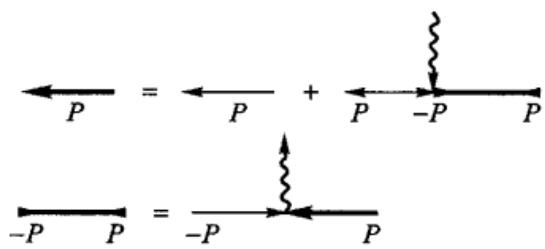
\includegraphics[width=8.2cm]{fig41_23.jpg}}
\tag{41.23}
\end{equation*}
其中细箭头对应于因子$\mathrm iG^{(0)}(P)$，$G^{(0)}(P)$是理想费米气体格林函数. 入射和出射于顶点的波纹线分别对应于因子$\mathrm ig\Xi$和$-\mathrm ig\Xi^{*}$. 将(41.23)式与(33.7)式进行比较，我们看到$\mathrm ig\Xi$,$-\mathrm ig\Xi^{*}$这两个因子对应于自能函数$\mathrm i\Sigma_{02}$和$\mathrm i\Sigma_{20}$，也就是说，它们是这两个量的一级近似. 应当指出，新的图元素（双向箭头和波纹线）只限于超流费米系统的图技术这一特殊性；与玻色系统情况不同，这里不出现“三叉”顶点. 因此这里图技术比用于超流玻色系统的要简单得多，并更接近于“通常”的图技术.

\section{超流费米气体的温度格林函数}

在§41中曾运用通常的“时间”格林函数来确定超流费米气体的能谱. 然而，对于解决更复杂的问题（首先是研究处于外场中系统的性质），用温度格林函数这一数学工具（А.\,А.\,Абрикосов, Л.\,П.\,Горьков, 1958）就更为方便.

温度函数$\mathcal G_{\alpha\beta}$和用于正常费米气体时一样，由公式(37.3)定义. 但温度函数$\mathcal F_{\alpha\beta}$和$\bar{\mathcal F}_{\alpha\beta}$（对应于时间函数$F_{\alpha\beta}$和$F^{+}_{\alpha\beta}$）是用类似于\eqref{41.3}式的公式来定义的：
\begin{equation}
\begin{aligned}
\mathcal F_{\alpha\beta}(\tau_1\bm r_1;\tau_2,\bm r_2)
&= \sum_m\langle m,N|\,\hat w\,T_\tau\,\hat\Psi^{\mathrm M}_{\alpha1}\hat\Psi^{\mathrm M}_{\beta2}\,|\,m,N+2\rangle\,,\\
\bar{\mathcal F}_{\alpha\beta}(\tau_1,\bm r_1;\tau_2,\bm r_2)
&= \sum_m\langle m,N+2|\,\hat w\,T_\tau\,\hat{\overline\Psi}^{\mathrm M}_{\alpha1}\hat{\overline\Psi}^{\mathrm M}_{\beta2}\,|\,m,N\rangle\,.
\end{aligned}
\label{42.1}
\end{equation}
这两个函数的自旋依赖关系以因子$g_{\alpha\beta}$［与\eqref{41.5}式一样］的形式分离出来\footnote{与(41.6)式中符号相同的情况不同，定义式中~$\mathcal F$与~$\bar{\mathcal F}$的符号相反是合理的，因为定义(42.1)没有(41.3)式中的因子~$\mathrm i$.}：
\begin{equation}
\mathcal F_{\alpha\beta} = g_{\alpha\beta}\mathcal F\,,\quad \bar{\mathcal F}_{\alpha\beta} = -g_{\alpha\beta}\bar{\mathcal F}\,.
\label{42.2}
\end{equation}
同$\mathcal G$一样，函数$\mathcal F$和$\bar{\mathcal F}$只与差值$\tau=\tau_1-\tau_2$有关，并遵从关系式(37.6)（取上面符号）：
\begin{equation}
\mathcal F(\tau) = -\mathcal F\Biggl(\tau+\frac{1}{T}\Biggr)\,,\quad
\bar{\mathcal F}(\tau) = -\bar{\mathcal F}\Biggl(\tau+\frac{1}{T}\Biggr).
\label{42.3}
\end{equation}
因此，这两个函数按$\tau$展开的傅里叶级数只包含奇数“频率”(37.8a)：$\zeta_s=(2s+1)\pi T$.

$\tau=0$时的松原$\psi$算符与$t=0$时的海森伯算符一致：
\begin{equation*}
\hat\Psi^{\mathrm M}(\tau=0,\bm r) = \hat\Psi(t=0,\bm r)\,.
\end{equation*}
将函数$\mathcal F$,$\bar{\mathcal F}$的定义同$F$,$F^{+}$的定义作对比，因此求得：
\begin{equation}
\mathcal F(0,\bm r;0,\bm r) = \Xi(\bm r)\,,\quad \bar{\mathcal F}(0,\bm r;0,\bm r) = \Xi^{*}(\bm r)\,.
\label{42.4}
\end{equation}
这里应把$\Xi$理解为按吉布斯分布求平均（即用系统温度表达）的凝聚体波函数.

现在我们证明，如何借助温度格林函数才能重新得出温度不等于零时的超流费米气体的能谱.

像推导方程\eqref{41.12}—\eqref{41.13}一样，我们可以推导出温度函数$\mathcal G$,$\mathcal F$和$\bar{\mathcal F}$的方程. 其中，把对$t$求微商换成对$\tau$求微商，而利用异于\eqref{41.8}—\eqref{41.9}（其中将$\mathrm it$换成$\tau$）的方程来代替它们. 像\eqref{41.11}式一样，从4个松原算符乘积的平均值中分解出含有粒子数改变2的跃迁矩阵元的各项. 结果我们得到方程：
\begin{equation}
\left\{
\begin{aligned}
&\Biggl(-\frac{\partial}{\partial\tau}+\frac{\nabla^2}{2m}+\mu\Biggr)\mathcal G(\tau,\bm r;\tau',\bm r')
+ g\Xi\bar{\mathcal F}(\tau,\bm r;\tau',\bm r') = {}\\
&\qquad = \delta(\tau-\tau')\,\delta(\bm r-\bm r')\\
&\Biggl(\frac{\partial}{\partial\tau}+\frac{\nabla^2}{2m}+\mu\Biggr)\bar{\mathcal F}(\tau,\bm r;\tau',\bm r')
- g\Xi^{*}\mathcal G(\tau,\bm r;\tau',\bm r') = 0
\end{aligned}
\right.
\label{42.5}
\end{equation}
转到傅里叶分量之后，这两个方程取如下形式：
\begin{equation}
\begin{aligned}
(\mathrm i\zeta_s-\eta_p)\mathcal G(\zeta_s,\bm p) + g\Xi\bar{\mathcal F}(\zeta_s,\bm p) &= 1\,,\\
-(\mathrm i\zeta_s+\eta_p)\bar{\mathcal F}(\zeta_s,\bm p) - g\Xi^{*}\mathcal G(\zeta_s,\bm p) &= 0\,.
\end{aligned}
\label{42.6}
\end{equation}
这两个方程的解：
\begin{equation}
\mathcal G(\zeta_s,\bm p) = -\frac{\mathrm i\zeta_s+\eta_p}{\zeta_s^2+\varepsilon^2}\,,
\label{42.7}
\end{equation}
\begin{equation}
\bar{\mathcal F}(\zeta_s,\bm p) = \frac{g\Xi^{*}}{\zeta_s^2+\varepsilon^2} = F^{+}(\mathrm i\zeta_s,\bm p)\,,
\label{42.8}
\end{equation}
这里又有$\varepsilon^2=\Delta^2+\eta_p^2$，$\Delta=g\Xi$（而且这个解是唯一确定的，它根本不包含函数$G$和$F^{+}$中的任何$\delta$函数）.

确定能谱中存在能隙的条件，现在可以从如下等式得出：
\begin{equation*}
\Xi^{*} = \bar{\mathcal F}(\tau=0,\bm r=0)
= T\sum_{s=-\infty}^{\infty}\int\bar{\mathcal F}(\zeta_s,\bm p)\,\frac{\mathrm d^3p}{(2\pi)^3}\,.
\end{equation*}
或代入\eqref{42.8}式后，得：
\begin{equation}
\frac{gT}{(2\pi)^3}\sum_{s=-\infty}^{\infty}\int\frac{\mathrm d^3p}{\zeta_s^2+\varepsilon^2(p)} = 1\,.
\label{42.9}
\end{equation}
为实行对$s$求和，可用公式\footnote{为得出这个公式，我们写出
\begin{equation*}
\frac{1}{(2s+1)^2\pi^2+a^2}=\frac{1}{2a}\Biggl[\frac{1}{a+\mathrm i\pi(2s+1)}+\frac{1}{a-\mathrm i\pi(2s+1)}\Biggr]
=\frac{1}{2a}\int_0^{\infty}\mathrm e^{-ax}\bigl[\mathrm e^{-\mathrm i\pi(2s+1)x}+\mathrm e^{\mathrm i\pi(2s+1)x}\bigr]\mathrm dx,
\end{equation*}
并在积分号下对几何级数求和即可.}：
\begin{equation}
\sum_{s=-\infty}^{\infty}\bigl[(2s+1)^2\pi^2+a^2\bigr]^{-1} = \frac{1}{2a}\tanh\frac{a}{2}\,,
\label{42.10}
\end{equation}
因而得出与\eqref{39.15}相同的等式：
\begin{equation}
\frac{g}{2}\int\frac{1}{\varepsilon}\tanh\frac{\varepsilon}{2T}\,\frac{\mathrm d^3p}{(2\pi)^3} = 1\,.
\label{42.11}
\end{equation}

\section{金属的超导性}

1911年由卡末林·昂内斯（H.\,Kamerlingh Onnes）发现的金属的超导现象乃是金属中电子费米液体的超流性，它类似于我们在前几节中所研究的简并费米气体的超流性. 虽然，在许多重要方面电子液体同费米气体是本质上不同的物理系统，但是与能谱性质有关的主要物理因素，在两种情况下仍然是相同的. 现在我们用定性的方式讨论这样一个问题：上边所研究的模型究竟有哪些特点，可以在多大程度上转用于金属中的电子.

金属的一个重要特性是，其电子的能谱是各向异性的，这与我们所研究的费米气体具有各向同性的能谱是相反的. 但是，这种情况并不妨碍库珀现象的产生，对于后者而言，一个极为重要的事实是：存在界限分明的费米面（不论其形状如何），而面上状态数密度都是有限的. 动量相反和自旋相反的电子必须具有
相同的能量，即两个电子应同位于一个费米面上. 这一要求，由于对时间反演的对称性而自然得到保证. 因此可以说，由于时间的相互反演而得出的各态中的电子都将配成对.

下一个问题是金属中电子相互作用的符号问题. 按最简化意义可以说，这种相互作用是由原子间距上受屏蔽的库仑排斥作用和通过晶格的相互作用形成的. 后一种相互作用，可描写为交换虚声子的结果，并具有吸引的性质（§64）. 如果这种相互作用“占优势”，金属在足够低的温度下将变成超导体.

重要的是，通过交换声子而相互作用的仅仅是处于费米面附近$\bm p$空间中较窄层内的那些电子；这个层的厚度$\sim\hbar\omega_{\mathrm D}$并小于电子的化学势$\mu$（$\omega_{\mathrm D}$是晶体的德拜频率）. 因此，若用弱非理想费米气体模型去描述超导性，则需要将\eqref{39.19}式中的截断参量$\tilde\varepsilon$理解为\footnote{因而积分(39.16)在大动量时发散的问题就消除了（对照150页上的注解）}：
\begin{equation}
\tilde\varepsilon\sim\hbar\omega_{\mathrm D}
\label{43.1}
\end{equation}
（做代替$\tilde\varepsilon\sim\mu$）.

至于说到相互作用微弱这一假设，实际上对于一切超导体都有
\begin{equation}
T_c\ll\hbar\omega_{\mathrm D}\ll\mu\,.
\label{43.2}
\end{equation}
但是，§39中所作的假设更强：耦合常数$g$是个小量，它使\eqref{39.19}式中量纲为1的指数函数的值变大. 现在这种要求可表成如下条件：
\begin{equation}
\ln(\hbar\omega_{\mathrm D}/T_c)\gg1\,.
\label{43.3}
\end{equation}
这里不仅比值$\hbar\omega_{\mathrm D}/T_c$要大，而且它的对数也必须大. 这个条件实际上未能得到很好的满足\footnote{比值~$\hbar\omega_{\mathrm D}/T_c$大约在对~Pb 为~10 到对~Al 和~Cd 为~300 的范围内变动.}.

考虑到金属中的电子液体与弱非理想费米气体模型的所有实际差别，超导理论就变得非常复杂了. 但同时发现，基于上述模型的简单理论，已经在许多方面对超导体的性质不仅定性地甚至定量地作出很好的描述. 前面已经提到，这个理论是由Bardeen，Cooper和Schrieffer建立的；因此，把粒子间呈现微弱吸引作用的费米气体模型，称作 BCS 模型.

上面讲到的这些都属于“普通的”或“低温的”超导体. 1986年贝德诺兹（J.\,G.\,Bednorz）和穆勒（K.\,A.\,M\"uller）发现新的一类物质——“高温超导体”. 这些物质多数是铜、稀土金属的氧化物，可有高的转变温度——高于$100\ \mathrm K$，而费米能并不高，为$1\,000\ \mathrm K$数量级. 但是，对这种有趣现象现在尚未建立较完整的理论、甚至对超导的相互作用本质也不完全清楚.

\section{超导电流}

在电中性超流液体（液氦）中有两种运动，它们对应于超导金属中能同时流动的两种电流. 超导电流不传热也不伴有能量耗散，因而它能在热力学平衡系统中产生；正常电流与释放焦耳热有关. 我们把超导电流密度和正常电流密度记为$\bm j_s$和$\bm j_n$；总电流密度$\bm j=\bm j_s+\bm j_n$.

只要从出现新的宏观量——凝聚体波函数$\Xi(t,\bm r)$这一事实本身出发，不论什么样的特殊模型都能对超导电流性质作出许多重要论断.

同§26节一样，我们引入函数$\Xi(t,\bm r)$的相位$\Phi$：
\begin{equation}
\Xi(t,\bm r) = |\Xi|\,\mathrm e^{\mathrm i\Phi}.
\label{44.1}
\end{equation}
就液氦来说，相位$\Phi$梯度按(26.12)式确定超流速度$\bm v_0$，与此类似，在超导体情况下相位梯度则确定观测量——超导电流密度. 由于金属是各向异性的，一般说来，$\bm j_s$的方向与$\nabla\Phi$的方向并不相同，而这两个矢量各分量之间的关系由某二阶张量确定. 但是，为避免非原则地复杂化起见，这里我们只局限于讨论金属晶体的立方对称情况.

这时，二阶张量归结为一个标量，而$\bm j_s$和$\nabla\Phi$之间的关系归结为简单的正比关系. 我们把它写成：
\begin{equation}
\bm j_s = \frac{e\hbar}{2m}\,n_s\,\nabla\Phi\,.
\label{44.2}
\end{equation}
按定义，这里$e=-|e|$是电子电荷，$m$为电子的真实质量. 这样定义的量$n_s$（温度的函数）称作超导电子数密度；该量在这里所起的作用，类似于液氦中的超流分量密度. 我们强调一下，$n_s$与库珀对凝聚体密度绝不是一回事，正像液氦中$\rho_s$不同于凝聚体原子密度\footnote{(44.2)式中写出的系数，在自由超流费米气体（BCS）模型中，可使~$mn_s$与§40中算出的量~$\rho_s$一致. $\rho_s$这样确定时，电流密度~$\bm j_s$应表达为~$\bm j_s=en_s\bm v_s$，式中~$\bm v_s$是超流运动速度. 至于~$\bm v_s$与相位梯度的关系，可用等式~$\bm v_s=(\hbar/2m)\nabla\Phi$来表达；这里二倍质量~$2m$［代换(26.12)式中的~$m$］，是因为凝聚体由成对粒子构成.}.

公式\eqref{44.2}［同液氦的公式(26.12)一样］要求在空间中相位的变化充分缓慢. 虽然，在玻色液体情况下只要求相位在原子间距上缓变，但在这里要求条件明显更强了. 相干长度$\xi_0\sim\hbar v_{\mathrm F}/\Delta_0$对超流费米液体起着特征线度的作用，相位$\Phi$在这个距离（大于原子间距）上应当有小的改变\footnote{应当强调，这里出现的恰好是与温度无关的恒定参量长度~$\xi_0$；以后将给出这个判据的严格论证（见§51的结尾）.}.

如果超导体处于外磁场中，则$\bm j_s$和$\Phi$之间的关系就复杂了；这里，我们研究$\bm j_s$和$\Phi$恒定场（对时间）的情况. 下面，需要对公式\eqref{44.2}加以必要的修改，对此可以从理论的规范不变性的要求出发进行说明.

这一要求是：一切被观测的物理量，在磁场矢势作规范变换：
\begin{equation}
\bm A\longrightarrow\bm A + \nabla\chi(\bm r)
\label{44.3}
\end{equation}
时，保持不变，式中$\chi(\bm r)$是任意坐标函数. 这时，$\psi$算符同波函数有相同的变换法则：
\begin{equation}
\hat\psi\longrightarrow\hat\psi\exp\Biggl(\frac{\mathrm ie}{\hbar c}\chi\Biggr),\quad
\hat\psi^{+}\longrightarrow\hat\psi^{+}\exp\Biggl(-\frac{\mathrm ie}{\hbar c}\chi\Biggr).
\label{44.4}
\end{equation}
式中$e$是用$\psi$算符描述的粒子的电荷（见第三卷(111.9)式）\footnote{由于在二次量子化的哈密顿量(7.7)中~$\psi$算符以~$\hat\Psi(X)$和~$\hat\Psi^{+}(X)$这样一对算符的形式出现，所以作(44.3—44.4)的变换时，上述哈密顿量的变换，就跟通常的（非算符的）波函数这样变换时通常的哈密顿量变换一样. (44.3—44.4)形式的变换，实际上在§19中就已经用过了.}. 作为乘积$\hat\Psi\hat\Psi^{+}$或$\hat\Psi\hat\Psi'$的矩阵元的格林函数$G(X,X')$和$F(X,X')$可按下式变换：
\begin{equation}
\begin{aligned}
G(X,X') &\to \exp\Biggl\{\frac{\mathrm ie}{\hbar c}\Bigl[\chi(\bm r)-\chi(\bm r')\Bigr]\Biggr\}G(X,X')\,,\\
F(X,X') &\to \exp\Biggl\{\frac{\mathrm ie}{\hbar c}\Bigl[\chi(\bm r)+\chi(\bm r')\Bigr]\Biggr\}F(X,X')\,.
\end{aligned}
\label{44.5}
\end{equation}
此时
\begin{equation*}
\Xi = \mathrm iF(X,X)\longrightarrow\exp\Biggl(\frac{2\mathrm ie}{\hbar c}\chi\Biggr)\Xi\,.
\end{equation*}
即凝聚体波函数的相位
\begin{equation}
\Phi\longrightarrow\Phi + \frac{2e}{\hbar c}\chi(\bm r).
\label{44.6}
\end{equation}
关系式\eqref{44.2}对这样的相位变换，并非是不变的. 为了达到所要求的不变性，此式应增加一个含磁场矢势的项：
\begin{equation}
\bm j_s = \frac{\hbar e}{2m}\,n_s\Biggl(\nabla\Phi - \frac{2e}{\hbar c}\bm A\Biggr)
\label{44.7}
\end{equation}
括号中第二项的二倍电荷，表示超导体的电子是成对出现的.

这个表达式，足以解释超导体的主要宏观性质——将磁场排出超导体之外［迈斯纳（Meissner）效应］\footnote{唯象超导体电动力学，在本教程的另一卷中讲述，见第八卷第六章.}.

我们现在研究处于弱磁场中的均匀超导体，这里假定磁场值小于破坏超导性的临界磁场$H_{\mathrm c}$. 这个条件，消除了磁场对$n_s$值的重要影响. 假设物体处于热力学平衡态，因此正常电流不存在了，故$\bm j=\bm j_s$\footnote{此后，在本章内各处都做这种假设，因此~$\bm j$在这里都是超导电流密度.}. 现在对等式\eqref{44.7}两边施行$\nabla\times$运算，并注意$\nabla\times\bm A=\bm B$——物体中的磁感应，我们便得到伦敦方程：
\begin{equation}
\nabla\times\bm j = -\frac{e^2n_s}{mc}\,\bm B
\label{44.8}
\end{equation}
（F.\,London, H.\,London, 1935）\footnote{上述方程(44.8)是~Л.\,Д.\,朗道推导的（1941）.}.

这是超导体特有的方程. 我们再用普遍的麦克斯韦方程：
\begin{equation}
\nabla\times\bm B = \frac{4\pi}{c}\,\bm j\,,
\label{44.9}
\end{equation}
\begin{equation}
\nabla\cdot\bm B = 0.
\label{44.10}
\end{equation}
将\eqref{44.9}式中的$\bm j$代入\eqref{44.8}式，并注意由于\eqref{44.10}式，$\nabla\times(\nabla\times)\bm B=-\Delta\bm B$，于是得到超导体中的磁场方程：
\begin{equation}
\Delta\bm B = \delta^{-2}\bm B
\label{44.11}
\end{equation}
式中引入记号
\begin{equation}
\delta^2 = mc^2/4\pi e^2n_s\,.
\label{44.12}
\end{equation}

我们利用这个方程来求超导体内靠近表面处场的分布，而这个表面看作平面；现在选取这个平面作为$yz$面，而$x$轴指向物体内部. 根据这些条件，场的分布只与一个坐标$x$有关，因而由\eqref{44.10}式我们有$\mathrm dB_x/\mathrm dx=0$；于是从\eqref{44.11}式自然得出$B_x=0$. 方程\eqref{44.11}现在具有$\mathrm d^2B/\mathrm dx^2=B/\delta^2$的形式，由此
\begin{equation}
\bm B(x) = \pmb{\mathfrak H}\,\mathrm e^{-x/\delta}\,,
\label{44.13}
\end{equation}
式中矢量$\pmb{\mathfrak H}$平行于表面.

我们看到，磁场向超导体深处按指数函数衰减，并只穿透$\sim\delta$的距离. 这个长度是宏观量，但小于大尺度样品的一般线度（$\delta\sim10^{-6}$—$10^{-5}\ \mathrm{cm}$），因此磁场实际上只穿透很薄的表面层. 长度$\delta$称作场的伦敦穿透深度. 应当强调，这个长度是一个直接可测的量，它具有完全确定的意义，这与参量$n_s$的约定意义是不同的.

但是上面所导出的结果，需要一个重要的附加条件. 出发的公式\eqref{44.7}，只在所有的物理量在空间作充分缓变的条件下才能适用：物理量在其间发生重大改变的特征距离，应当远远大于相干长度$\xi_0$\footnote{我们提醒一下，磁感应~$\bm B$本身是按物理无限小的体积元求平均的真实微观磁场强度，各体积元的尺度仅大于晶格常数.}. 就是说，在这种情况下应有
\begin{equation}
\delta\gg\xi_0.
\label{44.14}
\end{equation}

当然，这一要求并不影响对于从超导体中排出磁场这一事实的证明，因为假如不排出磁场会导致逻辑上的矛盾. 本来，在这种情况下磁场的变化是非常缓慢的，于是方程\eqref{44.11}就会适用. 但具体的方程\eqref{44.11}以及由它得出的场的衰减规律\eqref{44.13}，只当遵从条件\eqref{44.14}时才成立.

在超导体中，当满足不等式$\delta\gg\xi_0$时，称作伦敦情况，在相反情况下当$\delta\ll\xi_0$时，叫做皮帕德（Pippard）情况（在这种情况下，磁场向超导体深处的衰减规律将在§52中研究）. 当$T\to T_c$时，超导电子密度$n_s\to0$，因此$\delta\to\infty$. 所以在充分接近转变点处，总是属于伦敦情况. 但当$T\to0$时，$\delta$和$\xi_0$之间的关系将依赖于金属的具体性质\footnote{例如，在周期系的过渡族纯金属及某些中间金属化合物中，在整个温度范围内都发生伦敦情况. 在非过渡族纯金属中，远离~$T_c$时发生皮帕德情况.}.

最后，我们还要研究表达式\eqref{44.7}的一个推论，它不依赖$\delta$和$\xi_0$之间的关系.

从宏观超导体电动力学我们知道，如果磁通量通过超导圆环的孔道，则这种通量在物体状态作任意变化（而不破坏它的超导性）时，始终是不变的；这时假定，超导圆环是大尺度的，它的直径和厚度大于相干长度和场的穿透深度. 现在证明，“冻”在圆环的孔道里磁通量值，只能是某一基本“通量量子”的整数倍（F.\,London, 1954）.

在物体深处（超出场的穿透范围）电流密度$\bm j=0$；但矢势不为零——只是它的旋度即磁感应强度$\bm B$等于零. 我们选取任一闭合回路$C$，它包围圆环的孔道并在远离物体表面的地方通过物体的内部；这样选取，可保证遵从公式\eqref{44.7}的适用条件——相位$\Phi$和势$\bm A$在空间的变化充分缓慢. 矢量$\bm A$沿回路$C$的环流与通过回路平面的磁感应通量（即通过圆环孔道的通量$\phi$）相等：
\begin{equation*}
\oint\bm A\cdot\mathrm d\bm l = \int(\nabla\times\bm A)\cdot\mathrm d\bm f = \int\bm B\cdot\mathrm d\bm f = \phi\,.
\end{equation*}
另一方面，使表达式\eqref{44.7}等于零，并把它沿回路进行积分，我们得到：
\begin{equation*}
\oint\bm A\cdot\mathrm d\bm l = \frac{\hbar c}{2e}\oint\nabla\Phi\cdot\mathrm d\bm l = \frac{\hbar c}{2e}\,\delta\Phi\,.
\end{equation*}
式中$\delta\Phi$是环绕回路时波函数相位的改变. 但由于要求这个函数具有单值性，因而相位的改变只能是$2\pi$的整数倍. 所以我们得出如下结果：
\begin{equation}
\phi = n\phi_0\,,\quad \phi_0 = \frac{\pi\hbar c}{|e|} = 2\times10^{-7}\ \mathrm{Gs}\cdot\mathrm{cm}^2\ \text{（高斯·厘米$^{2}$）}.
\label{44.15}
\end{equation}
式中$n$是整数. $\phi_0$值是基本磁通量子.

磁通量的量子化也有另外一方面的涵义：它将导致总电流$\bm J$发生离散值，而$\bm J$在无外场时可以流过超导环. 事实上，电流$J$产生通过圆环孔道的磁通量，其值等于$LJ/c$，这里$L$是自感系数. 使这个通量等于$n\phi_0$，便求得电流的可能值：
\begin{equation}
\bm J = \frac{c\phi_0}{L}\,n = \frac{\pi\hbar c^2}{|e|L}\,n.
\label{44.16}
\end{equation}
与磁通量子相反，“总电流量子”同自感$L$一起依赖于圆环的形状和大小.

\begin{xiti}

试求磁场中半径为$R\ll\delta$的超导小球在伦敦情况下的磁矩.

{\heiti 解：}当$R\ll\delta$时，可以认为球内磁场是恒定的，并等于外场$\pmb{\mathfrak H}$. 如果选取矢势为$\bm A=\frac12\,\pmb{\mathfrak H}\times\bm r$，则可简单取
\begin{equation*}
\bm j = -(n_se^2/mc)\,\bm A\,,
\end{equation*}
［即取\eqref{44.7}式中的$\Phi=0$］；这时，在球表面上电流正常成分的消失（$\bm n\cdot\bm j=0$）的边界条件自然得到满足. 磁矩可按如下积分算出：
\begin{equation*}
\bm M = \frac{1}{2c}\int\bm r\times\bm j\,\mathrm dV\,,
\end{equation*}
沿球的体积求积分后，便得：
\begin{equation*}
\bm M = -\frac{R^5}{30\delta^2}\,\pmb{\mathfrak H}\,.
\end{equation*}

\end{xiti}

\section{金兹堡-朗道方程}

描述磁场中超导体行为的完整理论，是非常复杂的. 但是在相变点附近的温度范围内，情况就大大简化了. 这里，有可能建立不仅适用于弱磁场也适用于强磁场的比较简单的方程组\footnote{下边所叙述的理论，属于金兹堡（В.\,Л.\,Гинзбург）和~Л.\,Д.\,朗道 1950 年的工作. 绝妙的是，这个理论在超导性微观理论出现以前就已经用唯象方法建立起来了.}.

在朗道第二级相变的一般理论中，“非对称”相与“对称”相的区别是用序参数描述的，此参数在相变点变为零（见第五卷§142）. 对于超导相来说，序参数自然就是凝聚体波函数$\Xi$. 从原则上看，为避免不必要的复杂化，我们把金属晶体看作是立方对称的；在§44中曾经指出，在这种情况下超导态是用标量$n_s$——超导电子密度来描述的. 对于这种情况，选择与$\Xi$成比例的量作为序参数更为方便，我们把这个量记为$\psi$，并遵从归一化条件$|\psi|^2=n_s/2$. $\psi$这个量的相位与函数$\Xi$的相位相同：
\begin{equation}
\psi = \sqrt{\frac{n_s}{2}}\,\mathrm e^{\mathrm i\Phi}.
\label{45.1}
\end{equation}
超导电流密度\eqref{44.2}，用$\psi$表达时可写成如下形式：
\begin{equation}
\bm j_s = \frac{e\hbar}{m}\,|\psi|^2\nabla\Phi
= -\frac{\mathrm ie\hbar}{2m}\bigl(\psi^{*}\nabla\psi - \psi\nabla\psi^{*}\bigr).
\label{45.2}
\end{equation}
该理论的出发点是：把超导体自由能表达成函数$\psi(\bm r)$的泛函. 根据朗道理论的一般原理，将自由能密度在相变点附近按微小的序参数$\psi$及其对坐标微商的幂展开，便可得到这个表达式. 下面我们首先研究无磁场情况下的超导体.

序参数$\psi$就其本身的意义来说，是与格林函数$F(X,X)\equiv-\mathrm i\Xi(X)$成比例的量，它不是单值函数：因为函数$F(X,X)$是由两个$\hat\Psi$算符构成的，所以任意改变这两个算符的相位，如$\hat\Psi\to\hat\Psi\mathrm e^{\mathrm i\alpha/2}$，都将使函数$F$的相位改变$\alpha$. 当然，物理量不应当依赖于这种任意性，也就是说，它们对于复序参数的变换$\psi\to\psi\mathrm e^{\mathrm i\alpha}$，应当是不变的. 有这一要求，就消除了自由能展开式中$\psi$的奇次方项.

这个展开式的具体形式，是按照第二级相变普遍理论（见第五卷§146）中的同样理由建立起来的. 这里不再重复这些讨论，我们直接写出超导体总自由能的如下展开式\footnote{我们只提醒一下，这里写出的梯度项的形式与假定晶体具有立方对称性有关. 在较低对称性的情况下，这一项就会有更一般的由微商~$\partial\psi/\partial x_i$构成的二次形式.}：
\begin{equation}
F = F_n + \int\Biggl\{\frac{\hbar^2}{4m}|\nabla\psi|^2 + a|\psi|^2 + \frac{b}{2}|\psi|^4\Biggr\}\,\mathrm dV\,,
\label{45.3}
\end{equation}
其中$F_n$是处于正常态（即$\psi=0$时）的自由能；$b$是只与物质密度有关（而与温度无关）的正系数；$a$值与温度的关系有如下规律：
\begin{equation}
a = (T-T_c)\,\alpha\,,
\label{45.4}
\end{equation}
并在相变点变成零；根据超导相对应于$T<T_c$的范围，所以系数$\alpha>0$；\eqref{45.3}式中$|\nabla\psi|^2$的系数是这样选定的：使电流具有表达式\eqref{45.2}的形式（见下面）\footnote{这种选择（其中包括视~$m$为电子的真实质量），当然没有什么深刻意义，其约定性与(44.2)式中定义~$n_s$的情形是一样的.}. 在\eqref{45.3}式中只出现$\psi$的一阶微商，这与$\psi$在空间作充分缓变的假设有关.

对于均匀超导体来说，在无外场的情况下，参数$\psi$与坐标无关. 这时，表达式\eqref{45.3}可化为
\begin{equation}
F = F_n + aV|\psi|^2 + \frac{bV}{2}|\psi|^4.
\label{45.5}
\end{equation}
当$T<T_c$时，$|\psi|^2$的平衡值决定于此表达式最小值的条件：
\begin{equation}
|\psi|^2 = -\frac{a}{b} = \frac{\alpha}{b}\bigl(T_c-T\bigr),
\label{45.6}
\end{equation}
即与温度有关的超导电子密度在相变点按线性规律变成零.

将\eqref{45.6}式的值代回\eqref{45.5}式，我们便求得超导态和正常态自由能的差：
\begin{equation}
F_s - F_n = -V\frac{\alpha^2}{2b}\bigl(T_c-T\bigr)^2.
\label{45.7}
\end{equation}
将此式对温度求微商，从而求得熵差，然后又可求出在相变点的热容量的跃变\footnote{将~$|\psi|^2=\rho_s/2m$的公式(45.6)和热容量跃变公式(45.8)与~BCS 模型中相同量的公式(40.16)和(40.11)作对比，便可以求出这个模型中的系数~$\alpha$和~$b$（Л.\,П.\,Горьков, 1959）：
\begin{equation*}
\alpha=6\pi^2T_c/7\zeta(3)\mu=7.04\times T_c/\mu\,,\qquad b=\alpha T_c/n.
\end{equation*}
这里利用了粒子数密度~$n=\rho/m$及化学势~$\mu$（当~$T=0$时）与理想气体边界动量的关系：
\begin{equation*}
n=p_{\mathrm F}^3/3\pi^2\hbar^3\,,\qquad \mu=p_{\mathrm F}^2/2m.
\end{equation*}}：
\begin{equation}
C_s - C_n = V\frac{\alpha^2T_c}{b}.
\label{45.8}
\end{equation}

在相变点附近，差式\eqref{45.7}乃是自由能的小附加量. 根据小附加量定理（第五卷§15）（表达成温度和压强的函数以代替温度和体积的函数）给出热力学势的差$\Phi_s-\Phi_n$. 另一方面，根据超导体热力学的一般公式［见第八卷(55.7)式］，这个差与$-VH_c^2/8\pi$的值相同，其中$H_c$是破坏超导性的临界场. 因此，我们求得在相变点附近临界场的温度依赖关系的如下规律\footnote{在~BCS 模型中：
\begin{equation*}
H_c=2.44\,(mp_{\mathrm F}/\hbar^3)^{1/2}(T_c-T)\,,\qquad \text{当~$T\to T_c$ 时；}
\end{equation*}
我们再得出这个模型中的~$T=0$时的~$H_c$值：
\begin{equation*}
H_c=0.99\,T_c\,(mp_{\mathrm F}/\hbar^3)^{1/2}.
\end{equation*}
［使(40.9)式的能量差等于~$-VH_c^2/8\pi$ 即得到此值］.}：
\begin{equation}
H_c = \Biggl(\frac{4\pi a^2}{b}\Biggr)^{1/2} = \Biggl(\frac{4\pi\alpha^2}{b}\Biggr)^{1/2}(T_c-T).
\label{45.9}
\end{equation}

在有磁场的情况下，自由能表达式\eqref{45.3}应当在两个方面加以改变. 第一，需要给被积式增加一项磁场能密度$\bm B^2/8\pi$（这里$\bm B=\nabla\times\bm A$是物体中的磁感应强度）. 第二，需要改变梯度项，以满足规范不变性的要求. 在上一节里曾经证明，这个条件将使凝聚体波函数的相位梯度$\nabla\Phi$必须代之以差$\nabla\Phi-(2e\bm A/\hbar c)$. 在此，是指需要作如下代换：
\begin{equation*}
\nabla\psi = \mathrm e^{\mathrm i\Phi}\nabla|\psi| + \mathrm i\psi\nabla\Phi
\longrightarrow \nabla\psi - \frac{2\mathrm ie}{\hbar c}\,\bm A\psi\,,
\end{equation*}
因此，我们得出如下的基本表达式：
\begin{equation}
\begin{aligned}
F = F_{n0} + \int\Biggl\{\frac{\bm B^2}{2\pi}
+ \frac{\hbar^2}{4m}\Biggl|\Biggl(\nabla - \frac{2\mathrm ie}{\hbar c}\bm A\Biggr)\psi\Biggr|^2
+ a|\psi|^2 + \frac{b}{2}|\psi|^4\Biggr\}\,\mathrm dV.
\end{aligned}
\label{45.10}
\end{equation}
（$F_{n0}$是无磁场时处于正常态的物体的自由能）. 应当强调，这个表达式中的系数$2\mathrm ie/\hbar c$不再有任意性（与上边指出的系数$\hbar^2/4m$的选择具有约定性不同）. 式中的二倍电子电荷是库珀对效应的结果（Л.\,П.\,Горьков, 1959）；当然，这个系数不可能用纯唯象方法确定出来.

现在，为寻求用以确定超导体中波函数$\psi$和磁场分布的微分方程，我们取作为三个独立函数$\psi$,$\psi^{*}$和$\bm A$的泛函的自由能极小值.

复量$\psi$是两个实量的集合；因此，在取变分时需要把$\psi$和$\psi^{*}$看作独立函数. 将积分对$\psi^{*}$取变分，并把$\bigl(\nabla\psi-2\mathrm ie\bm A/\hbar c\bigr)\nabla\delta\psi^{*}$项的积分作变换后进行分部积分，我们得到：
\begin{equation}
\begin{aligned}
\delta F = \int\Biggl\{-\frac{\hbar^2}{4m}\Biggl(\nabla - \frac{2\mathrm ie}{\hbar c}\bm A\Biggr)^2\psi
+ a\psi + b|\psi|^2\psi\Biggr\}\delta\psi^{*}\,\mathrm dV + {}\\
+\ \frac{\hbar^2}{4m}\oint\Biggl(\nabla\psi - \frac{2\mathrm ie}{\hbar c}\bm A\psi\Biggr)\delta\psi^{*}\cdot\mathrm d\bm f\,.
\end{aligned}
\label{45.11}
\end{equation}
第二个积分是沿物体表面取的. 令$\delta F=0$，对于任意的$\delta\psi^{*}$，作为体积积分等于零的条件，我们得到如下方程：
\begin{equation}
\frac{1}{4m}\Biggl(-\mathrm i\hbar\nabla - \frac{2e}{c}\,\bm A\Biggr)^2\psi + a\psi + b|\psi|^2\psi = 0
\label{45.12}
\end{equation}
（再把积分对$\psi$取变分时，将得到它的复共轭方程，就是说给不出任何新的结果）.

同样地，把积分对$\bm A$取变分可得到麦克斯韦方程：
\begin{equation}
\nabla\times\bm B = \frac{4\pi}{c}\,\bm j\,,
\label{45.13}
\end{equation}
其中电流密度由下式给出：
\begin{equation}
\bm j = -\frac{\mathrm ie\hbar}{2m}\bigl(\psi^{*}\nabla\psi - \psi\nabla\psi^{*}\bigr)
- \frac{2e^2}{mc}\,|\psi|^2\bm A.
\label{45.14}
\end{equation}
此式与\eqref{44.7}式是一致的（我们写出$\bm j$以代替$\bm j_s$，因为在热力学平衡时不存在正常电流）. 应当注意，由\eqref{45.13}式得出连续性方程$\nabla\cdot\bm j=0$；考虑到方程\eqref{45.12}，直接微分\eqref{45.14}式也可以得出这个方程.

方程\eqref{45.12}—\eqref{45.14}组成了完整的金兹堡-朗道方程组.

这些方程的边界条件，可根据变分$\delta F$中沿物体表面的积分等于零的条件得出. 因此，由\eqref{45.11}式便得到边界条件：
\begin{equation}
\bm n\cdot\Biggl(-\mathrm i\hbar\nabla\psi - \frac{2e}{c}\,\bm A\psi\Biggr) = 0,
\label{45.15}
\end{equation}
式中$\bm n$是物体表面的法向矢量. 应注意，由于这个条件，\eqref{45.14}式的电流法向分量当然也应当变为零：$\bm n\cdot\bm j=0$\footnote{在(45.15)式的边界条件下，~$\psi$本身并不变成零，看来对于物体边界上的波函数来说，当然应该如此. 这种情况与下述原因有关：实际上~$\psi$只在距表面为原子尺度的距离上才变到零；其实，这样的距离在金兹堡-朗道理论中是看作可以忽略的小量.（详见~P.\,G.\,德让《金属与合金的超导性》. 俄文版为~Де Жен. Сверхпроводимость металлов и сплавов. — м.: мир, 1968, с.\,230--232.）
这里导出的条件(45.15)，实质上适用于超导体与真空的边界. 此条件对于超导体与电介质的边界仍然有效，但对于不同金属（其中，一个是超导金属，另一个是正常金属）之间的分界面是不适用的——在这个条件中没有考虑超导电子对正常金属的局部穿透效应. 在这种情况下，(45.15)式需要换成与~$\bm n\cdot\bm j=0$相容的具有更一般形式的条件：
\begin{equation*}
\bm n\cdot\Biggl(-\mathrm i\hbar\nabla\psi-\frac{2e}{c}\bm A\psi\Biggr)=\frac{\mathrm i\psi}{\lambda}.
\tag{45.15a}
\end{equation*}
式中~$\lambda$是实常数（具有长度量纲）；但是对这个常数的估计，则要求更详细的微观的探讨.}.

至于场的边界条件，则根据方程\eqref{45.13}，并考虑在整个空间（一直到物体表面为止）电流密度$\bm j$的有限性，可得出磁感应强度切向分量$B_t$具有连续性. 再从方程
\begin{equation*}
\nabla\cdot\bm B = 0
\end{equation*}
得出磁感应强度法向分量$B_n$的连续性. 换言之，边界条件要求整个矢量$\bm B$是连续的.

在弱磁场中可以忽略磁场对$|\psi|^2$的影响，并认为\eqref{45.6}式的$|\psi|^2$在物体各点等于常数值. 于是把\eqref{45.14}式代入\eqref{45.13}式（随后对方程两边施行$\nabla\times$运算）便得到伦敦方程\eqref{44.11}，其中穿透深度
\begin{equation}
\delta = \Biggl[\frac{mc^2b}{8\pi e^2|a|}\Biggr]^{1/2}
= \Biggl[\frac{mc^2b}{8\pi e^2\alpha(T_c-T)}\Biggr]^{1/2}.
\label{45.16}
\end{equation}
除此长度之外，金兹堡-朗道方程还包含一个特征长度：无磁场时序参数$\psi$的涨落关联半径；我们把它记为$\xi(T)$. 根据已知的涨落理论公式（见第五卷§146），此半径可用自由能\eqref{45.3}中的系数表达出来：
\begin{equation}
\xi(T) = \frac{\hbar}{2(m|a|)^{1/2}} = \frac{\hbar}{2(m\alpha)^{1/2}(T_c-T)^{1/2}}.
\label{45.17}
\end{equation}

金兹堡-朗道方程所描写的序参数$\psi$和磁场发生重要变化的距离，其数量级由特征长度\eqref{45.16}—\eqref{45.17}确定. 这时，一般来说$\delta$是磁场的特征长度，而$\xi(T)$是$\psi$分布的特征长度. 这两个长度应当远远大于“束缚对尺度”$\xi_0$，以满足所有物理量在空间作充分缓变的假设. 因为当按$(T_c-T)^{-1/2}$的规律趋于相变点时这两个长度增大，所以在相变点附近，一般地说这个条件可被满足（见下文）.

在所讨论的理论中，金兹堡-朗道参数起着重要作用，它定义为上述两个长度之比、是与温度无关的常数：
\begin{equation}
\kappa = \frac{\delta(T)}{\xi(T)} = \frac{mcb^{1/2}}{(2\pi)^{1/2}|e|\hbar}.
\label{45.18}
\end{equation}
按数量级来说，$\kappa\sim\delta_0/\xi_0$，这里$\xi_0$是相干长度\eqref{39.21}，$\delta_0$为绝对零度时伦敦穿透深度. 同时我们还指出，公式
\begin{equation}
\kappa = 2\sqrt2\,\frac{|e|}{\hbar c}\,H_c(T)\,\delta^2(T)
\label{45.19}
\end{equation}
是借助\eqref{45.9}和\eqref{45.16}式得出的，$\kappa$是直接通过观测量表达的.

各方程的形式已经建立，我们现在来讨论它们的适用范围.

从低温方面来看，方程的适用范围无论如何要受条件$T_c-T\ll T_c$的限制，这也是把序参数视为小量的条件，因而是把自由能进行全部展开的基础. 这个条件保证了遵从不等式$\xi(T)\gg\xi_0$，但在参数$\kappa$值小的超导体而又遵守不等式$\delta(T)\gg\xi_0$的情况下，条件是比较苛刻些\footnote{作为例子，我们引用几个纯金属的~$\kappa$值：Al---0.01, Sn---0.13, Hg---0.16, Pb---0.23.}；在这些情况下，从不等式$\delta\gg\xi_0$可得到如下条件：
\begin{equation}
T_c - T \ll \kappa^2 T_c.
\label{45.20}
\end{equation}

从$T\to T_c$方面来看，方程的适用性只受朗道的相变理论一般适用条件的限制，这个条件与序参数涨落的增大有关. 然而，此时这个条件是非常弱的. 实际上，用展开式\eqref{45.3}的系数可以把条件表达成如下不等式：
\begin{equation*}
T_c - T \gg \frac{b^2T_c^2}{\alpha(\hbar^2/m)^3}
\end{equation*}
（见第五卷(146.15)）. 例如，借助 BCS 模型中的$b$和$\alpha$值估算不等式右边的表达式，得：
\begin{equation}
(T_c-T)/T_c \gg (T_c/\mu)^4.
\label{45.21}
\end{equation}
由于比值$T_c/\mu\sim10^{-3}$—$10^{-4}$非常小，可以认为实际上一直到相变点都满足这个条件. 而超导相和正常相之间的第二级相变的涨落区实际上是不存在的.

\begin{xiti}

有厚度为$d\ll\xi,\delta$的平面膜，求平行于平面膜并可使超导性遭到破坏的磁场的临界值（В.\,Л.\,金兹堡, Л.\,Д.\,朗道, 1950）\footnote{关于小球的同样问题，见§47.}.

{\heiti 解：}我们选取膜的中间平面作为$xz$面，其中$x$轴沿磁场方向. 在场$\bm B\equiv B_z(y)$（沿垂直膜的$y$轴变化）的方程\eqref{45.13}中，可以认为$\psi=$ 常数. 于是电流表达式\eqref{45.14}中的第一项消去了，因而对\eqref{45.13}式施行$\nabla\times$运算便得到方程$B''=\theta^2B/\delta^2$，其中$\theta=\psi/\psi_0$，$\psi_0^2=|a|/b$，这个方程对$y$的对称解：
\begin{equation*}
B(y) = \pmb{\mathfrak H}\,\frac{\cosh(y\theta/\delta)}{\cosh(d\theta/2\delta)}
\approx \pmb{\mathfrak H}\Biggl[1 + \frac{y^2-(d/2)^2}{2\delta^2}\,\theta^2\Biggr]
\end{equation*}
（$\pmb{\mathfrak H}$是外场）. 这个场对应于电流的分布
\begin{equation*}
j = j_z = -\frac{c}{4\pi}\,B' \approx -\frac{c\theta^2\mathfrak H}{4\pi\delta^2}\,y.
\end{equation*}
但方程\eqref{45.12}中，$\psi$对$y$的依赖关系不能完全忽略，因为小的微商$\partial^2\psi/\partial y^2$在这里实际上要乘以$\hbar/m|a|\sim\xi^2$，因而具有大的因子$(\xi/d)^2$（由于条件$d\ll\xi$）；此时在这个方程中却可以忽略势$A=A_z(y)$，因为它将导致小量$d/\xi$的更高次项. 为了避免研究$\psi$对$y$的依赖关系，我们把方程\eqref{45.12}对膜的厚度求平均；这时对$y$的微商由于膜表面上的边界条件$\partial\psi/\partial y=0$而消失了. 再注意：
\begin{equation*}
-\frac{\partial^2\psi}{\partial z^2} \approx \Biggl(\frac{mj}{|e|\hbar|\psi|^2}\Biggr)^2\psi.
\end{equation*}
因为函数$\psi$的相位与$z$有关（以及$\psi$的梯度与电流的联系），所以用$\psi$约简后，得：
\begin{equation*}
\frac{m\overline{j^2}}{4e^2|\psi|^4} - |a| + b|\psi|^2 = 0.
\end{equation*}
式中
\begin{equation*}
\overline{j^2} = \frac{1}{d}\int_{-d/2}^{d/2}j^2\,\mathrm dy
= \frac{c^2d^2\theta^4\mathfrak H^2}{3(8\pi)^2\delta^4}.
\end{equation*}
再利用表达式\eqref{45.9}和\eqref{45.16}，便得到方程
\begin{equation*}
\frac{1}{24}\Biggl(\frac{\mathfrak H d}{H_c\,\delta}\Biggr)^2 = 1 - \frac{|\psi|^2}{\psi_0^2}.
\end{equation*}
此式确定了磁场中膜的$\psi$值. $\psi$为零时的场值，就是膜的临界场值$H_c^{\,f}$，它与大尺度超导体的临界场$H_c$的关系有如下等式：
\begin{equation*}
H_c^{\,f} = \sqrt{24}\,H_c\delta/d.
\end{equation*}
在我们所研究的条件下，磁场破坏超导性是借助于第二级相变，因为随$\pmb{\mathfrak H}$连续增大时$\psi$就变成零. 这是完全自然的，因为$d\ll\delta$时磁场实际上会穿透超导膜，所以不存在发生第一级相变的原因，而这第一级相变恰恰是场突然穿透物体时发生的.

\end{xiti}